\chapter{データセット}
本研究ではレスキュー犬訓練データセットのマルチクラス推定を行う.
訓練動画を用いる前に,犬一人称視点動画から行動分類が可能かどうかを確認するため簡易な予備実験を行なった.

また,本実験には現在作成中のサイバーレスキュー犬の訓練データセットを用いた.
既存の公開されている犬一人称視点動画データセットにDogCentric Actibity Dataset(DCAD)\cite{yumi2014first}がある.
予備実験にはDCADを用いた.

\section{サイバーレスキュー犬 訓練データセット}
サイバーレスキュー犬訓練データは,訓練されているレスキュー犬に,専用の計測スーツを着用させ収集したデータ群である(図~\ref{concat_movie}).
東北大学の大野らによって作成され,本研究ではその一部の提供を受けた.
現在も作成中であり,完成していないデータを含めた全てを使用することは困難である.
そのため,本研究ではその一部の提供されたデータをこれとして取り扱うものとする.
これは約2分から20分の7本の音声付き動画からなり,犬の一人称視点動画に加えてハンドラー視点動画,レスキュー犬とハンドラーを映す第三者視点動画が含まれる.本研究では犬の一人称視点動画のみを用いて推定を行う.
総時間は57分40秒,秒間フレーム数は29.97,総フレーム数は103696枚である.
分類クラスそれぞれについて時間範囲を指定する形で動画にアノテーションがされており,同時刻に複数のクラスが重なるためマルチラベルデータとして取り扱う.
例えば,「被災者を発見しながら吠えている」間はsee victimクラスとbarkクラスの2つのラベルが付与されている.
本研究ではこのデータを整形したものをサイバーレスキュー犬訓練データセットとして実験を行なった.最終的に利用したデータのクラス毎の出現頻度が~表\ref{cyberdataset_label}の値である.
動画は犬一人称視点のみを用いたが,犬一人称,ハンドラー視点,第三者視点毎にそれぞれラベル付けされたアノテーション情報に関しては全てを用いて学習を行った.
以下にデータにラベル付けされたクラスと,整形したデータについて詳細を述べる.
\begin{table}[H]
 \centering
 \caption{サイバーレスキュー犬訓練データセット 利用範囲内で計測した出現回数}\label{cyberdataset_label}
 \scalebox{0.95}[0.95]{
  \begin{tabular}{|l||c|c|c|c|c|c|c|c|c|c|c|}
   \hline \hline
      クラス   & \rotatebox{90}{bark}& \rotatebox{90}{cling}&\rotatebox{90}{command}& \rotatebox{90}{eat}&\rotatebox{90}{handler}& \rotatebox{90}{run}&\rotatebox{90}{victim}& \rotatebox{90}{shake}& \rotatebox{90}{sniff}& \rotatebox{90}{stop}& \rotatebox{90}{walk} \\ \hline

%   ラベル & bark&cling&comm&eat&handler&run&victim&shake&sniff&stop&walk \\ \hline
   出現回数& 1744& 1127&2439&343&  2011& 98&  1549&  239& 7719&6384&8764 \\ \hline
  \end{tabular}
 }

\end{table}


\subsection{分類クラス詳細}
各クラスについて説明する.
静止画のみでの音声付き動画のクラス特徴の表現は困難であるため、整形した動画的特徴,音声的特徴とをそれぞれに示す.
\begin{enumerate}
\item{bark}
被災者を発見し,かつ吠えている状態.わかりやすい音声的特徴があり,固有の画面揺れが生じる(図~\ref{bark}).
\item{cling}
臭いに対し,鼻を近づけ嗅いでいる状態.sniffのより詳細な状態であり,clingがラベル付される際はsniffと必ず重複する(図~\ref{cling}).
\item{command}
ハンドラーからの働きかけのある状態.待て/行け等の口頭指示,褒め,指差し指示など状況が多様である(図~\ref{command}).
\item{eat-drink}
何かを食べている/飲んでいる状態.訓練において被災者発見に対する成功報酬に餌が与えられる他,草を食む,地面/川の水を飲むなど状況が多様(図~\ref{eat-drink}).
以下,eatと表記する.特筆がない場合,eatという表記はeat(食事)とdrink(水分摂取)の両方の意,drinkという表記は水分摂取の意のみ表現する.
\item{look at handler}
犬がハンドラーを見ている状態(図~\ref{lookathandler}).
以下,handlerと表記する.
\item{run}
走っている状態.歩いているクラスのwalk-trotと比較すると,画面に浮遊感があり,揺れや音が激しい(図~\ref{run}).
\item{see victim}
カメラに被災者が映った状態(図~\ref{seevictim}).
以下,victimと表記する.
\item{shake}
犬が激しく体を震わせている状態.振動に合わせてカラカラカラとカメラの揺れる音がする(図~\ref{shake}).
\item{sniff}
臭いを嗅いでいる状態.探査に対するやる気などを測る一つに指標になる.地面などに鼻を近づけている状態だけでなく,浮遊臭を嗅いでいる際も含む(図~\ref{sniff}).
\item{stop}
足を運んでいない状態.その場での足踏みは含む.方向転換は含まない.画面の動き情報が少なく特徴的である(図~\ref{stop}).
\item{walk-trot}
歩いており、runではない状態(図~\ref{walk-trot}).第三者視点で見ると,犬の運歩がrunクラスとは異なる.
runクラスは前脚と後ろ脚で跳び箱を跳ぶように跳ねて進むが,walk-trotクラスは右左の脚を交互に出して進む.
以下,walkと表記する.
\begin{end}
\begin{figure}[H]
%  \begin{center}
    \begin{tabular}{c}
      \begin{minipage}{0.18\hsize}
        \begin{center}
          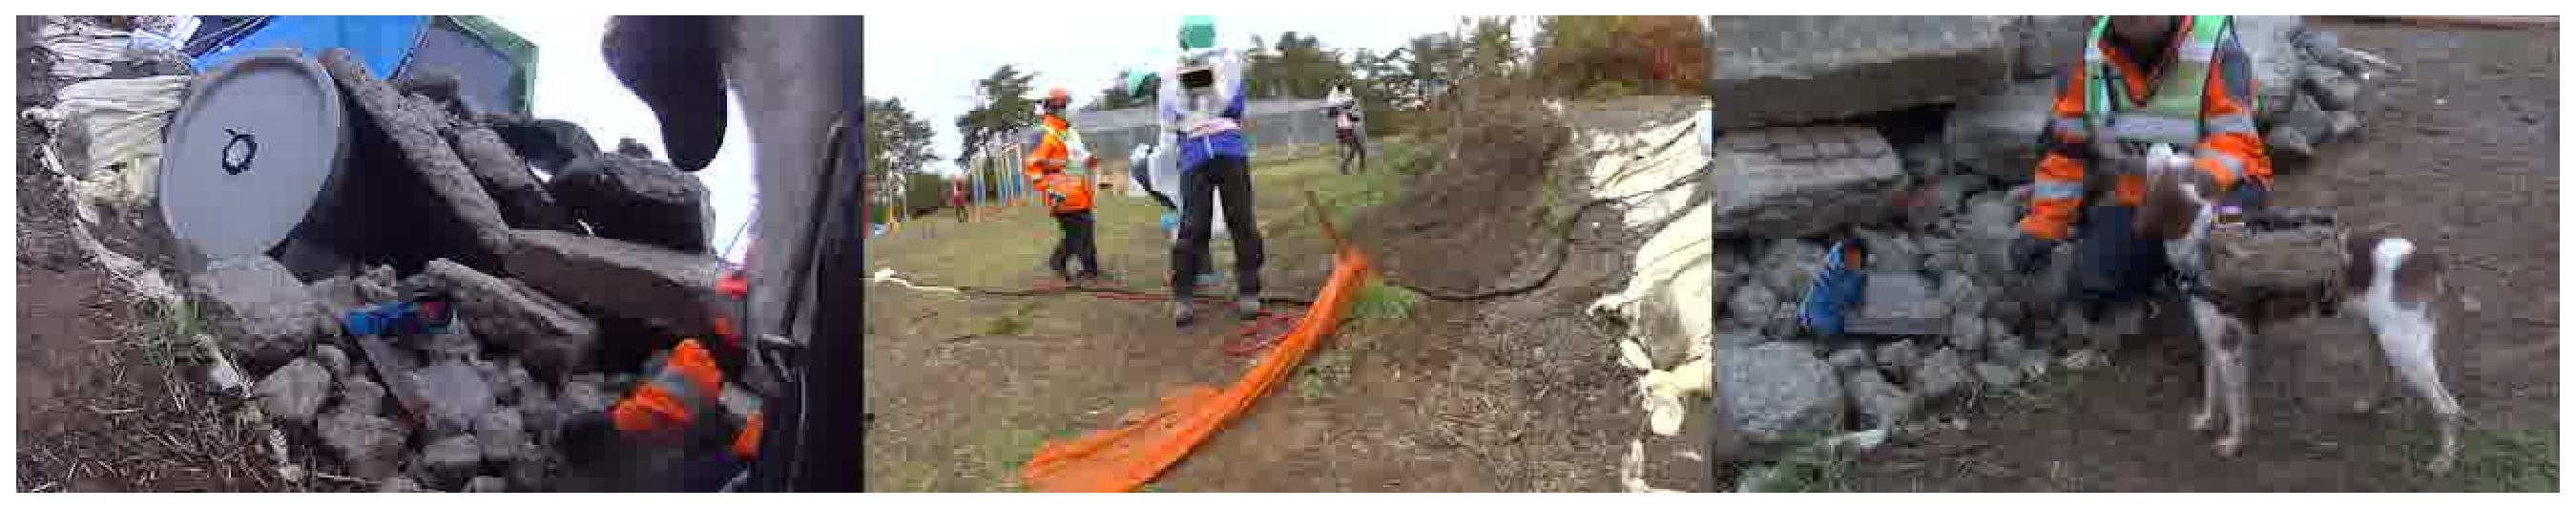
\includegraphics[clip, width=12cm]{./Figures/2016_gonta_1.eps}
          %\hspace{0.3cm} { }
        \end{center}
      \end{minipage}
\\
      \begin{minipage}{0.18\hsize}
        \begin{center}
          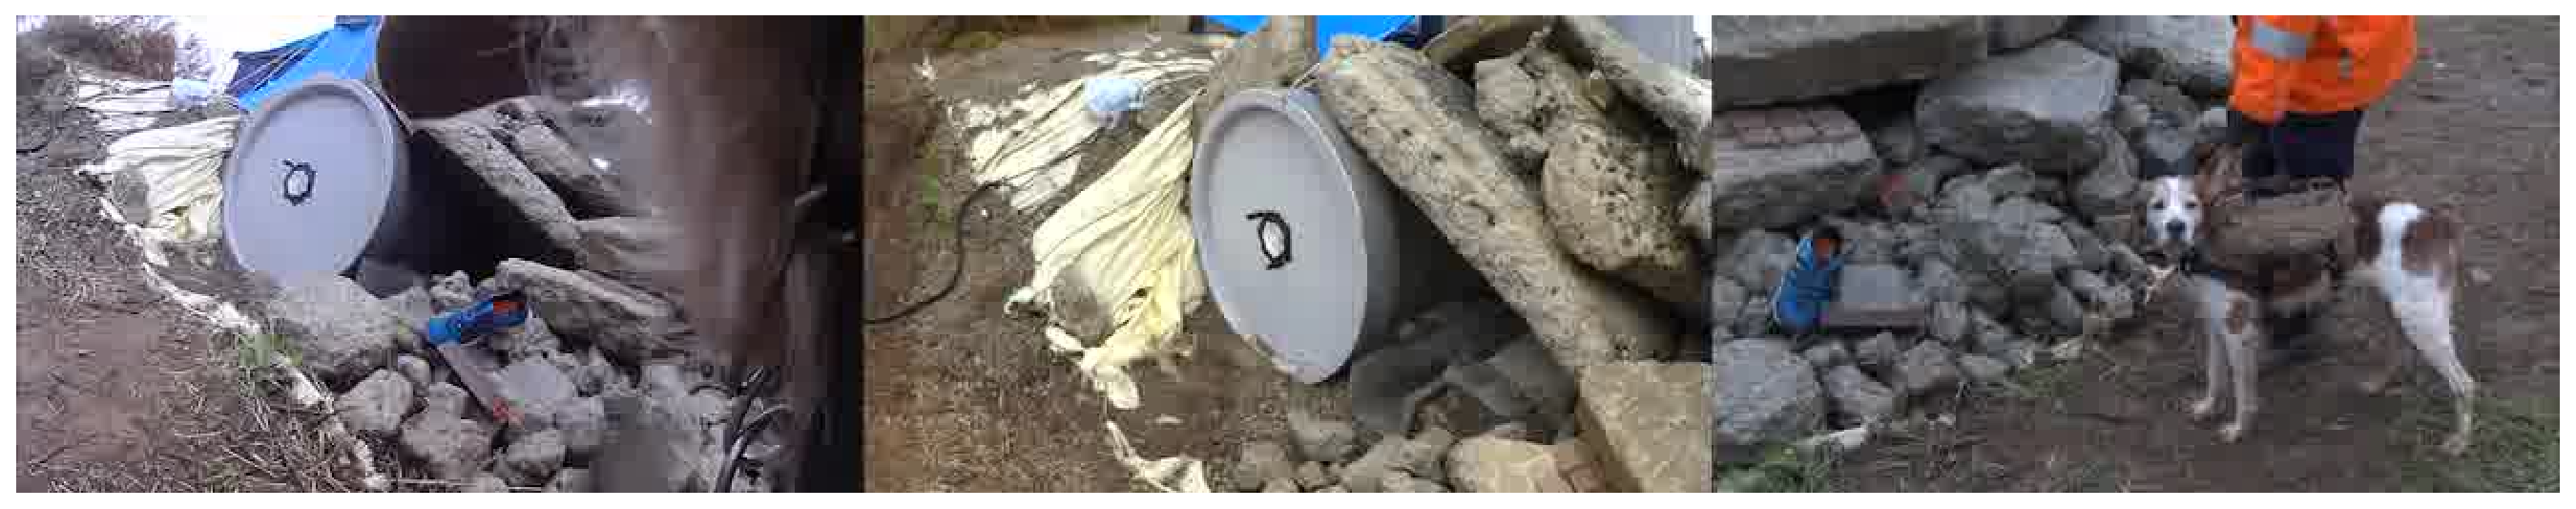
\includegraphics[clip, width=12cm]{./Figures/2016_gonta_2.eps}
          %\hspace{0.3cm} { }
        \end{center}
      \end{minipage}
\\
      \begin{minipage}{0.18\hsize}
        \begin{center}
          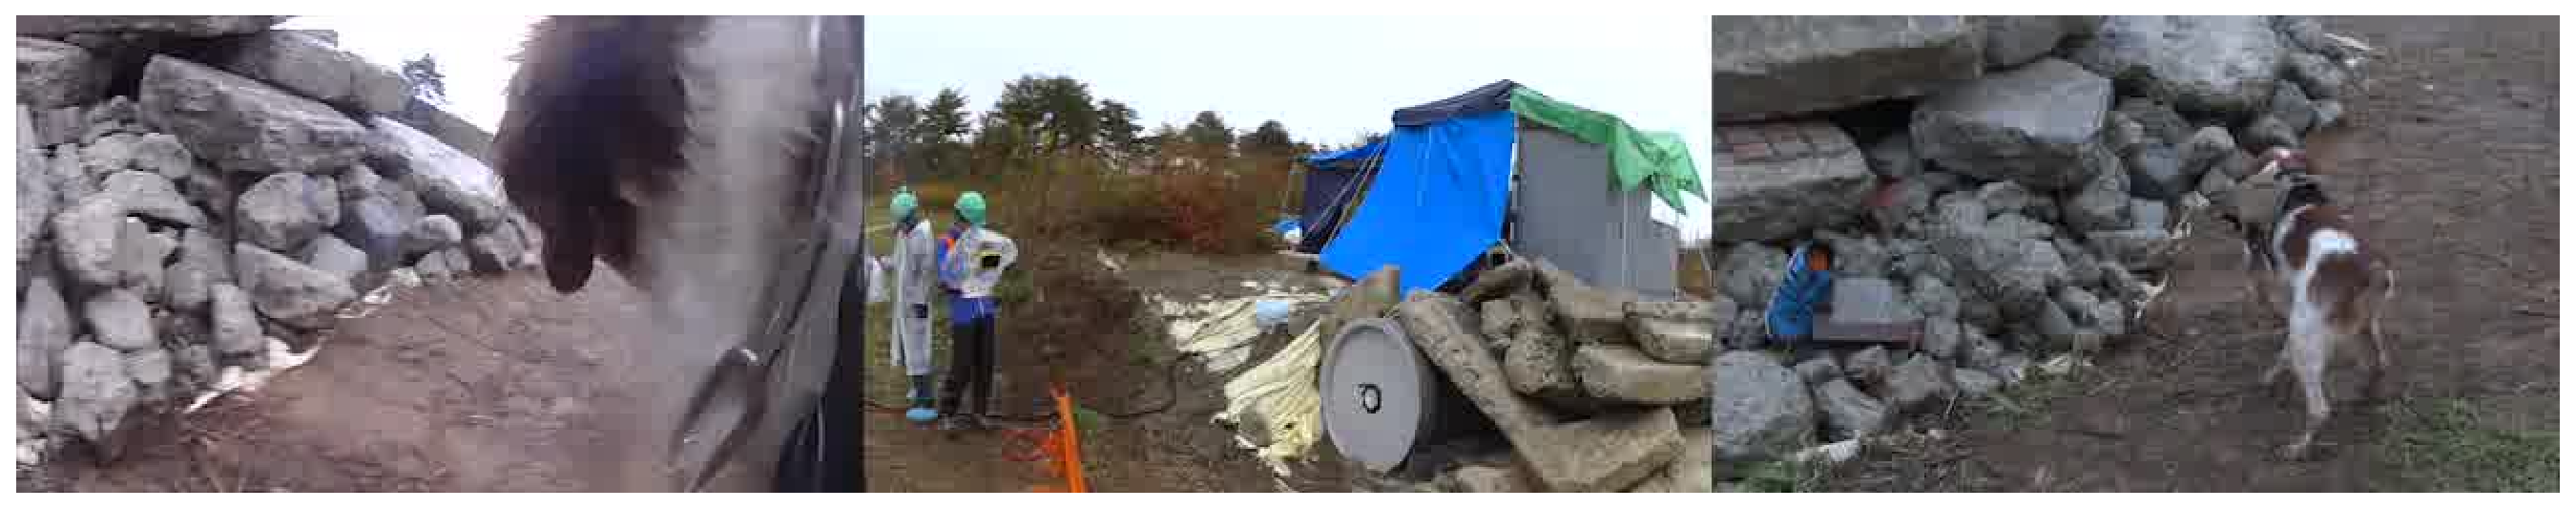
\includegraphics[clip, width=12cm]{./Figures/2016_gonta_3.eps}
          %\hspace{0.3cm} { }
        \end{center}
      \end{minipage}
\\
      \begin{minipage}{0.18\hsize}
        \begin{center}
          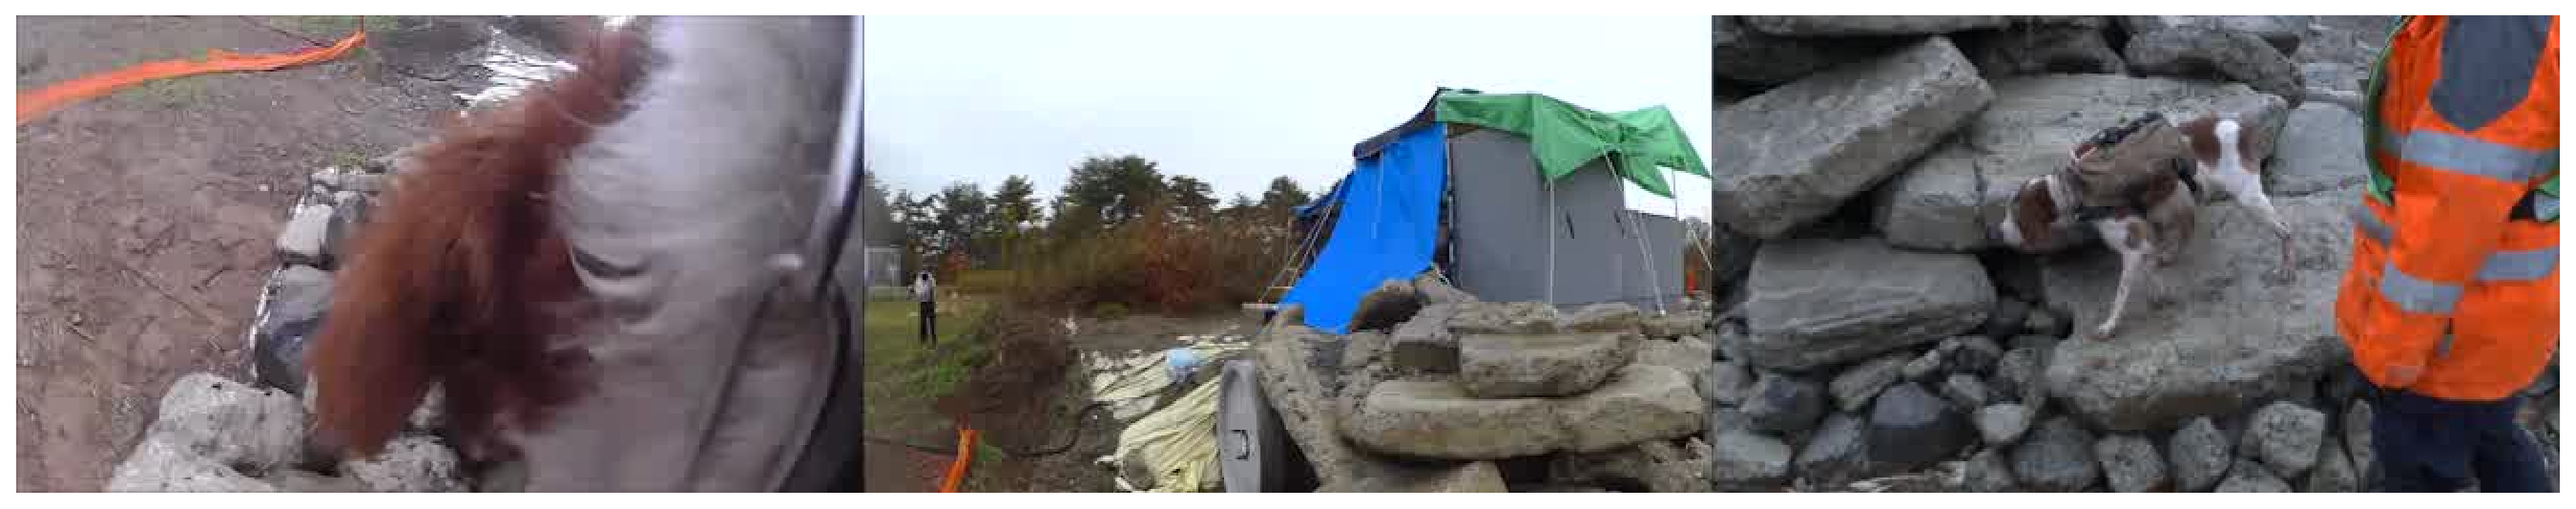
\includegraphics[clip, width=12cm]{./Figures/2016_gonta_4.eps}
          %\hspace{0.3cm} { }
        \end{center}
      \end{minipage}
\\
      \begin{minipage}{0.18\hsize}
        \begin{center}
          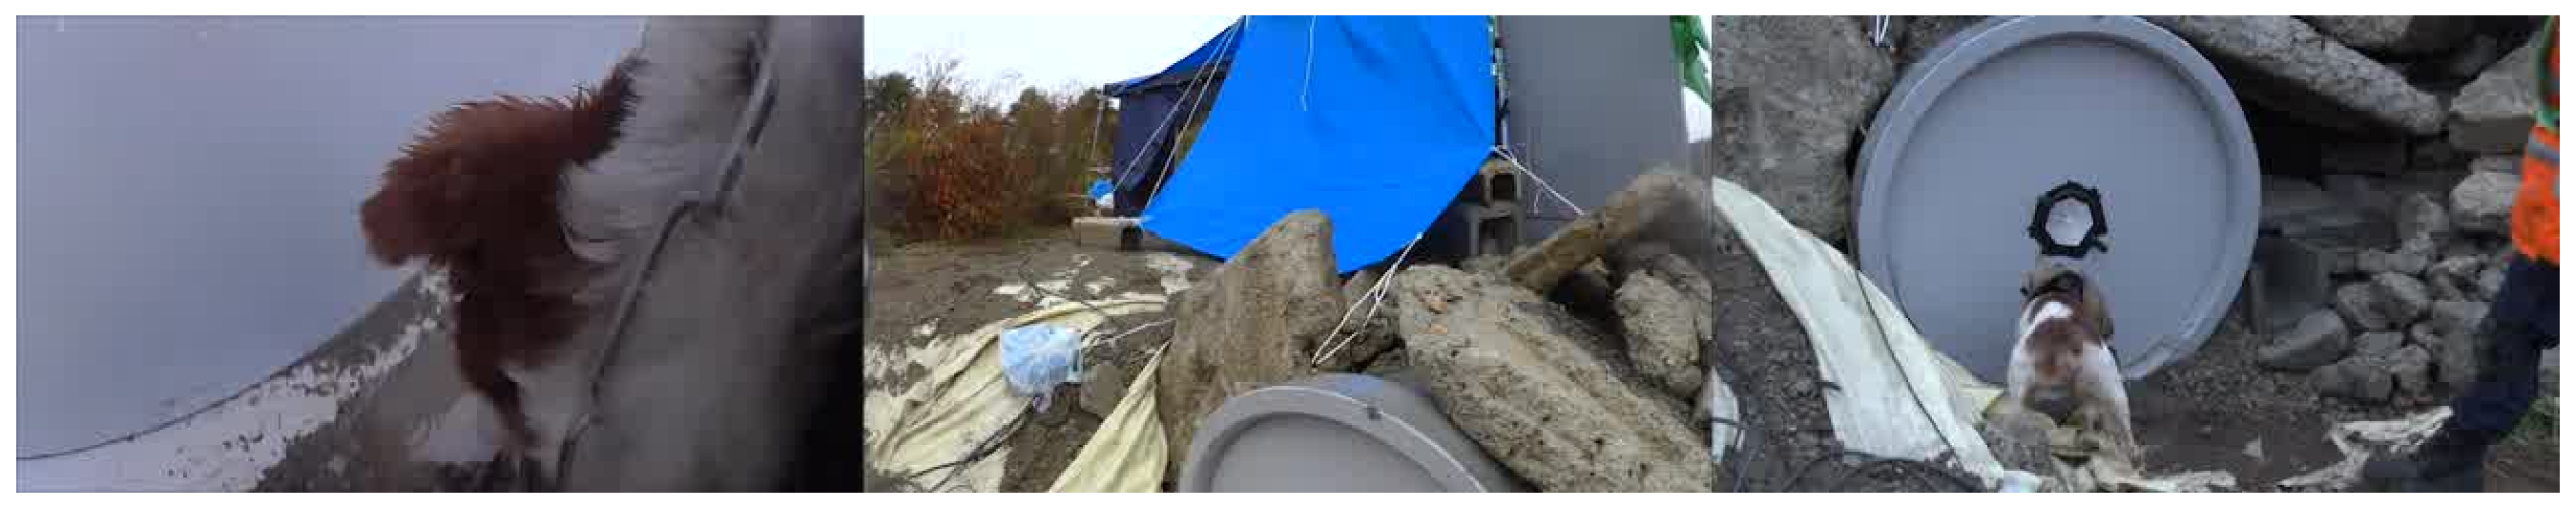
\includegraphics[clip, width=12cm]{./Figures/2016_gonta_5.eps}
          %\hspace{0.3cm} { }
        \end{center}
      \end{minipage}
    \end{tabular}
    \caption{提供時のデータ.左から,犬一人称視点,ハンドラー視点,第三者視点の動画が結合されている.合わせて1280x240pixelで,犬一人称視点だけ切り出しても通常カメラで撮影される比率にはならない.}
    \label{concat_movie}
%  \end{center}
\end{figure}


\begin{figure}[H]
    \begin{tabular}{l}
     % 0
      \begin{minipage}{0.165\hsize}
        \begin{center}
          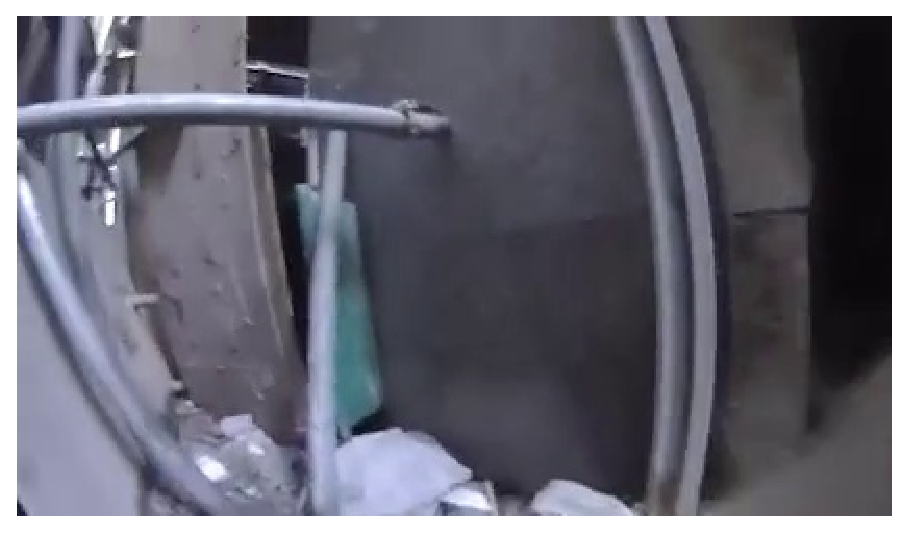
\includegraphics[clip, width=2.5cm]{./Figures/still_bark1.eps}
        \end{center}
      \end{minipage}
      \begin{minipage}{0.165\hsize}
        \begin{center}
          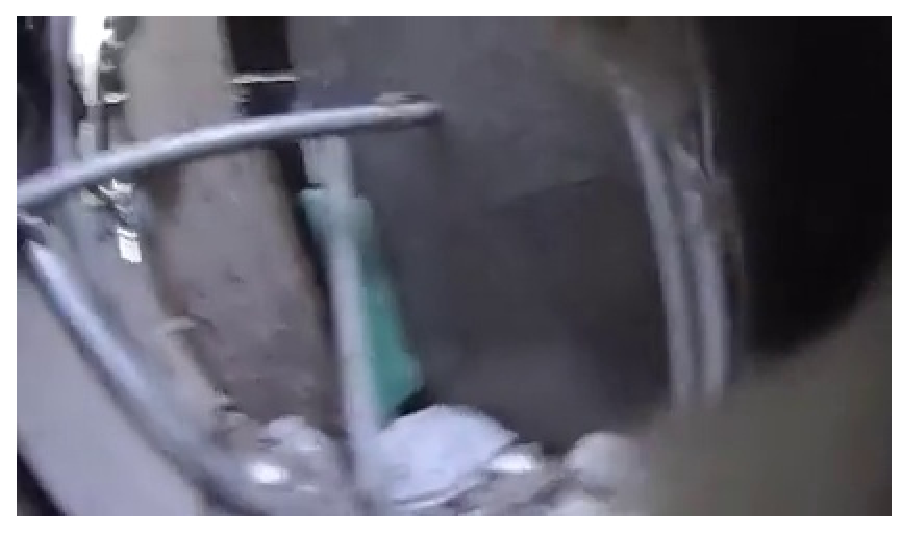
\includegraphics[clip, width=2.5cm]{./Figures/still_bark2.eps}
        \end{center}
      \end{minipage}
      \begin{minipage}{0.165\hsize}
        \begin{center}
          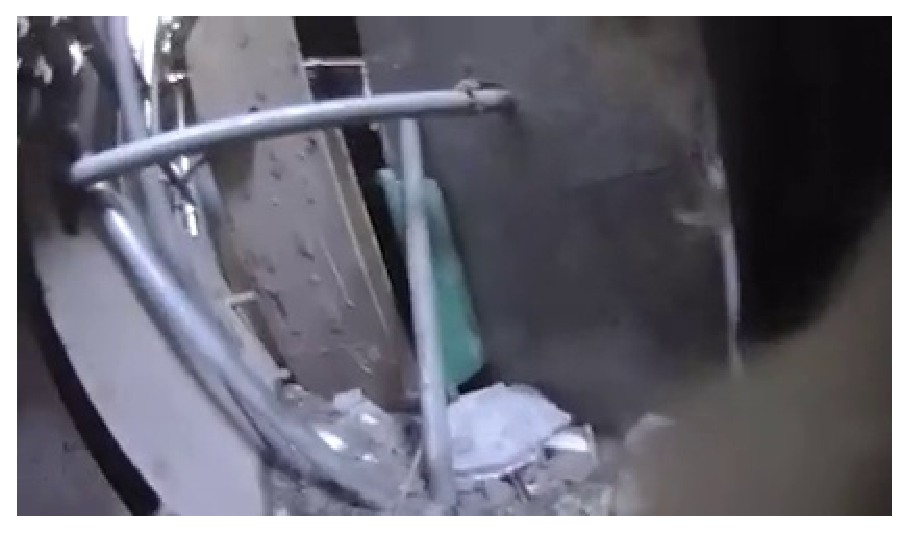
\includegraphics[clip, width=2.5cm]{./Figures/still_bark3.eps}
        \end{center}
      \end{minipage}
      \begin{minipage}{0.165\hsize}
        \begin{center}
          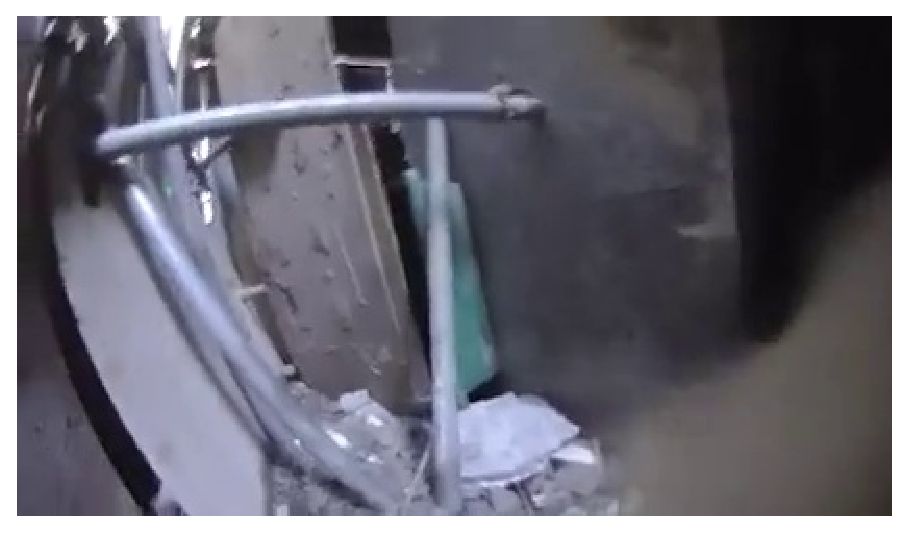
\includegraphics[clip, width=2.5cm]{./Figures/still_bark4.eps}
        \end{center}
      \end{minipage}
      \begin{minipage}{0.165\hsize}
        \begin{center}
          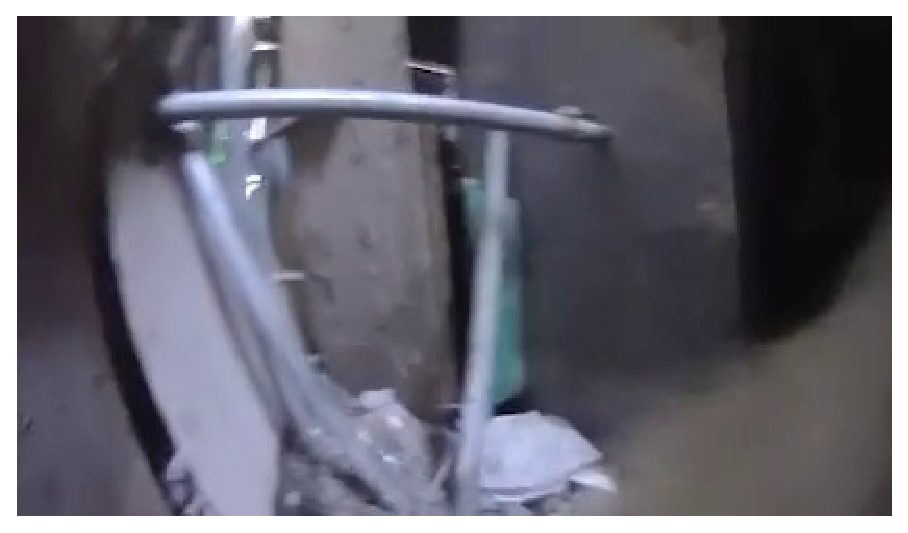
\includegraphics[clip, width=2.5cm]{./Figures/still_bark5.eps}
        \end{center}
      \end{minipage}
      \begin{minipage}{0.165\hsize}
        \begin{center}
          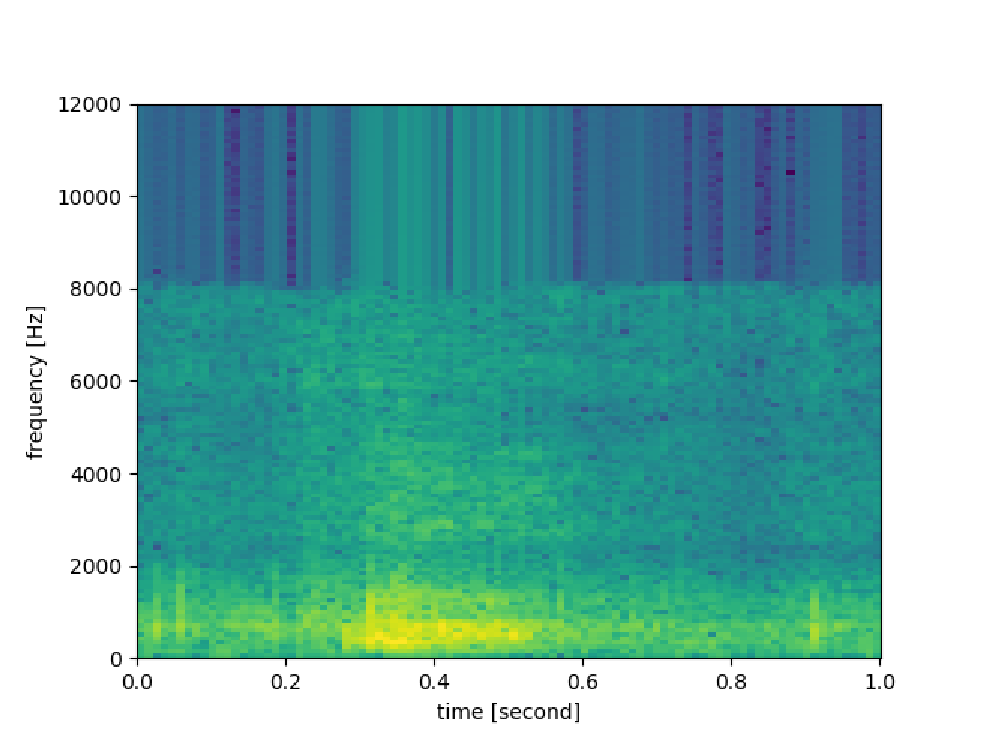
\includegraphics[clip, width=2.5cm]{./Figures/sound_bark.eps}
        \end{center}
      \end{minipage}
\\  %%%%%%%%%%%%%%%%
      \begin{minipage}{0.165\hsize}
        \begin{center}
          
\includegraphics[clip, width=2.5cm]{./Figures/optic_bark1.eps}
          \hspace{0.3cm} { }
        \end{center}
      \end{minipage}
      \begin{minipage}{0.165\hsize}
        \begin{center}
          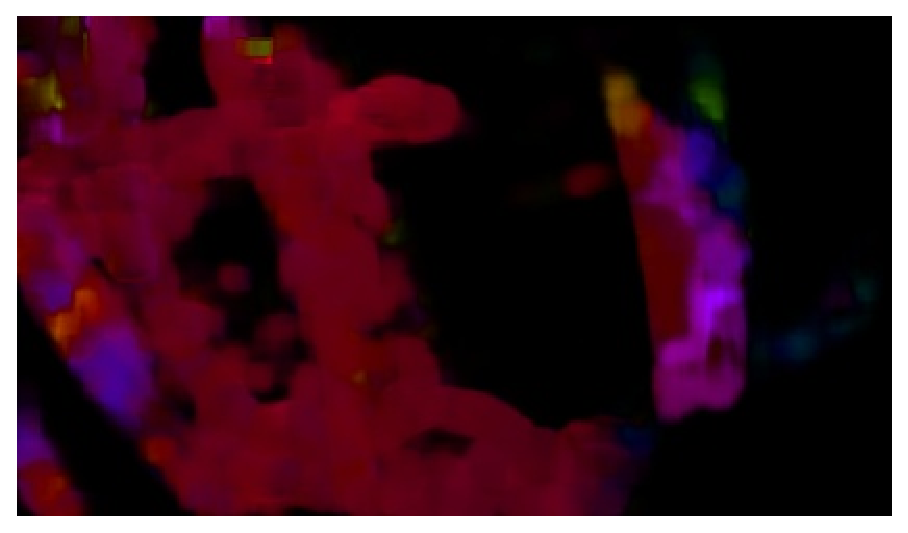
\includegraphics[clip, width=2.5cm]{./Figures/optic_bark2.eps}
          \hspace{0.0cm} { }
        \end{center}
      \end{minipage}
      \begin{minipage}{0.165\hsize}
        \begin{center}
          
\includegraphics[clip, width=2.5cm]{./Figures/optic_bark3.eps}
          \hspace{0.0cm} {bark}
        \end{center}
      \end{minipage}
      \begin{minipage}{0.165\hsize}
        \begin{center}
          
\includegraphics[clip, width=2.5cm]{./Figures/optic_bark4.eps}
          \hspace{0.1cm} { }
        \end{center}
      \end{minipage}
      \begin{minipage}{0.165\hsize}
        \begin{center}
          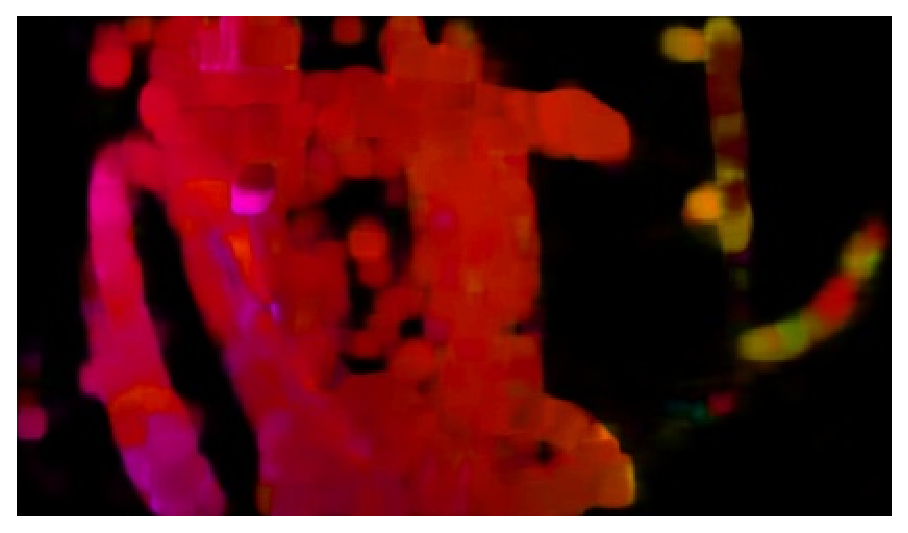
\includegraphics[clip, width=2.5cm]{./Figures/optic_bark5.eps}
          \hspace{2.2cm} { }
        \end{center}
      \end{minipage}
    \end{tabular}
    \caption{サイバーレスキュー犬訓練データセットbarkクラス}
    \label{bark}
\end{figure}

\begin{figure}[H]
    \begin{tabular}{l}

\\ %%%%%%%%%%%%%%%%%%%%%%%%%%%%%%%%%%

      \begin{minipage}{0.165\hsize}
        \begin{center}
          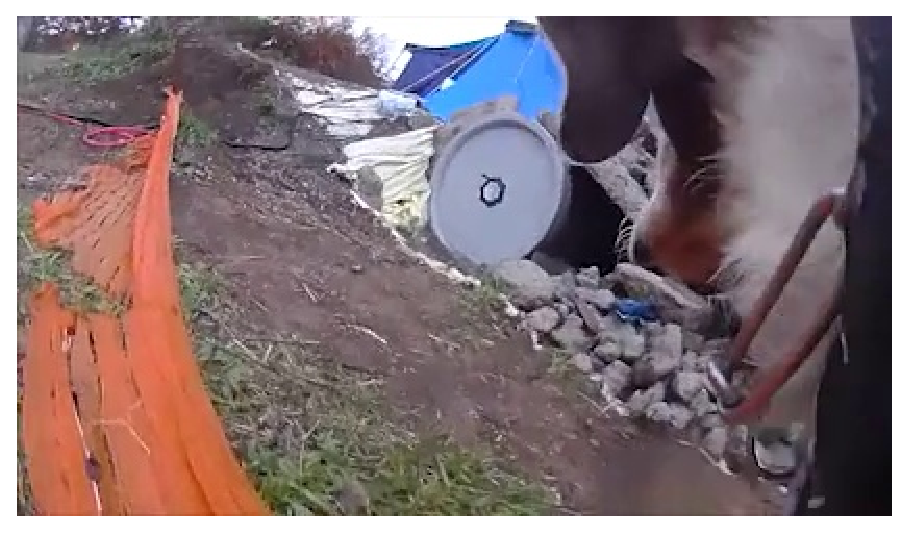
\includegraphics[clip, width=2.5cm]{./Figures/still_commandmatemate1.eps}
        \end{center}
      \end{minipage}
      \begin{minipage}{0.165\hsize}
        \begin{center}
          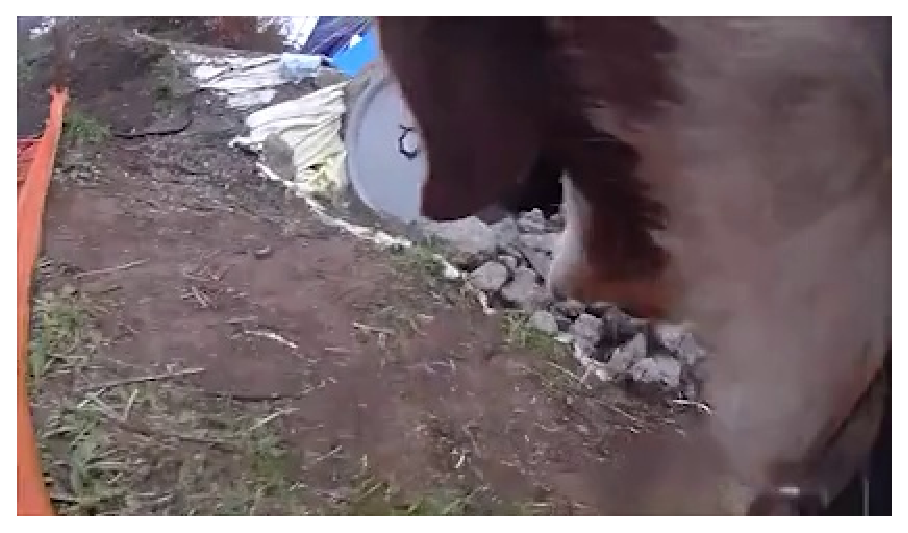
\includegraphics[clip, width=2.5cm]{./Figures/still_commandmatemate2.eps}
        \end{center}
      \end{minipage}
      \begin{minipage}{0.165\hsize}
        \begin{center}
          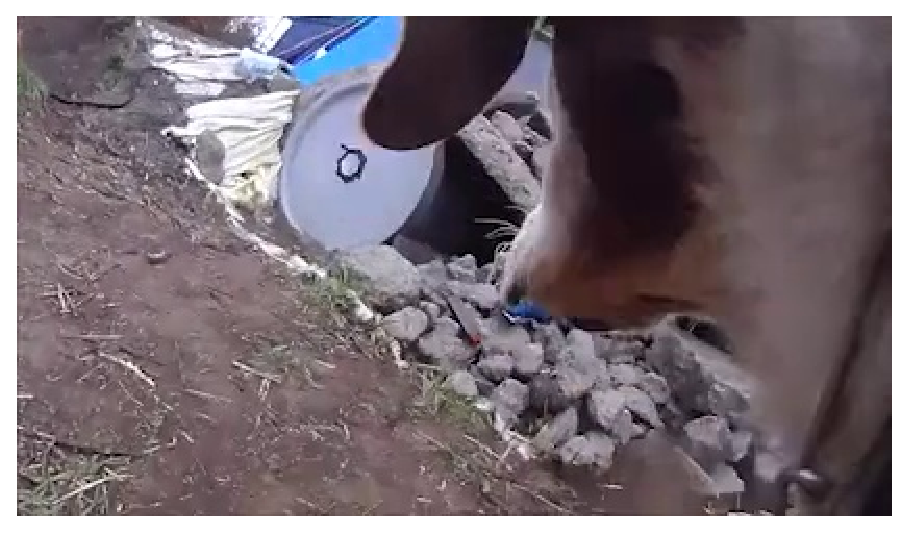
\includegraphics[clip, width=2.5cm]{./Figures/still_commandmatemate3.eps}
        \end{center}
      \end{minipage}
      \begin{minipage}{0.165\hsize}
        \begin{center}
          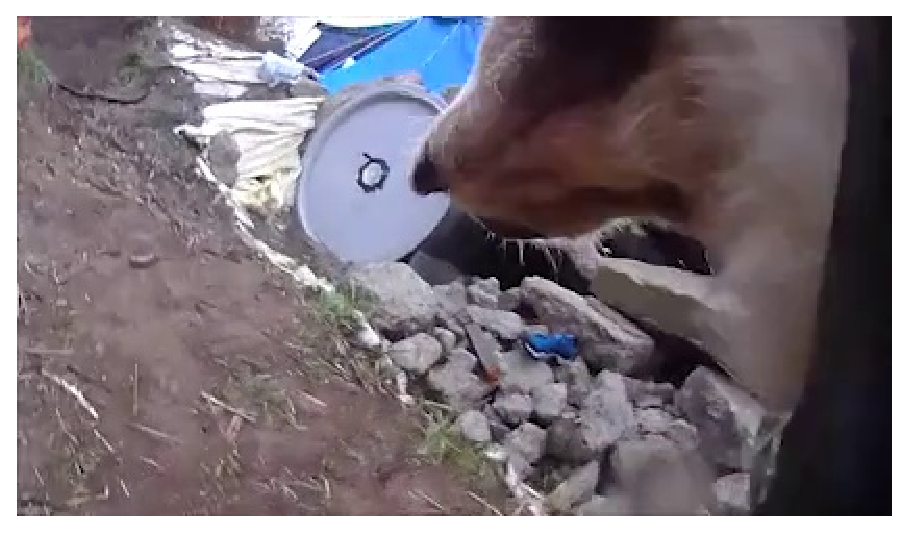
\includegraphics[clip, width=2.5cm]{./Figures/still_commandmatemate4.eps}
        \end{center}
      \end{minipage}
      \begin{minipage}{0.165\hsize}
        \begin{center}
          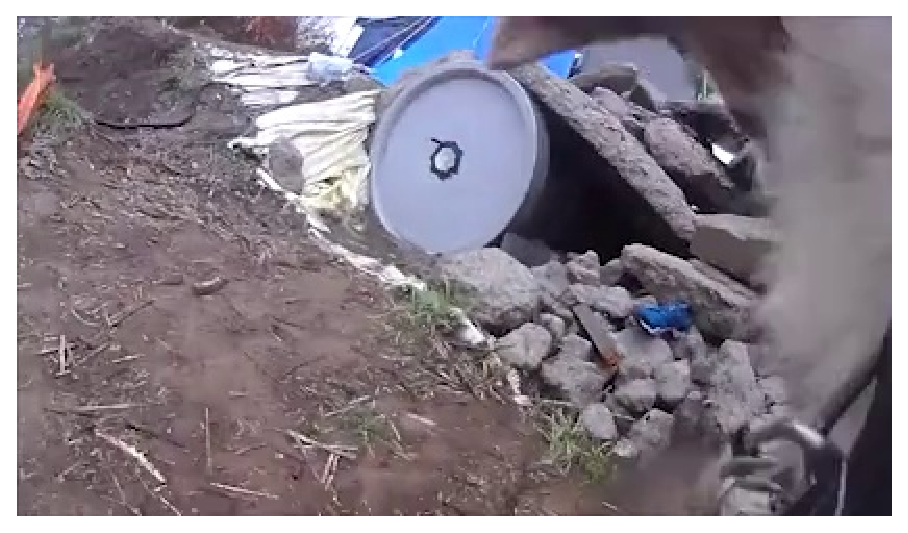
\includegraphics[clip, width=2.5cm]{./Figures/still_commandmatemate5.eps}
        \end{center}
      \end{minipage}
      \begin{minipage}{0.165\hsize}
        \begin{center}
          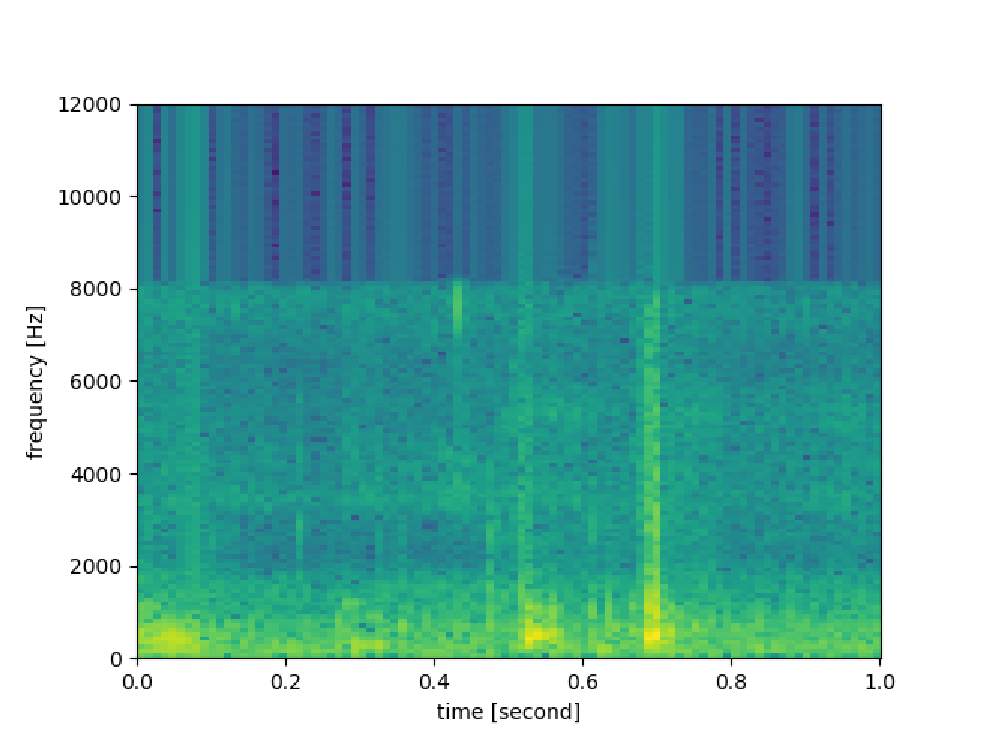
\includegraphics[clip, width=2.5cm]{./Figures/sound_commandmatemate.eps}
        \end{center}
      \end{minipage}
\\  %%%%%%%%%%%%%%%%
      \begin{minipage}{0.165\hsize}
        \begin{center}
          
\includegraphics[clip, width=2.5cm]{./Figures/optic_commandmatemate1.eps}
          \hspace{0.3cm} { }
        \end{center}
      \end{minipage}
      \begin{minipage}{0.165\hsize}
        \begin{center}
          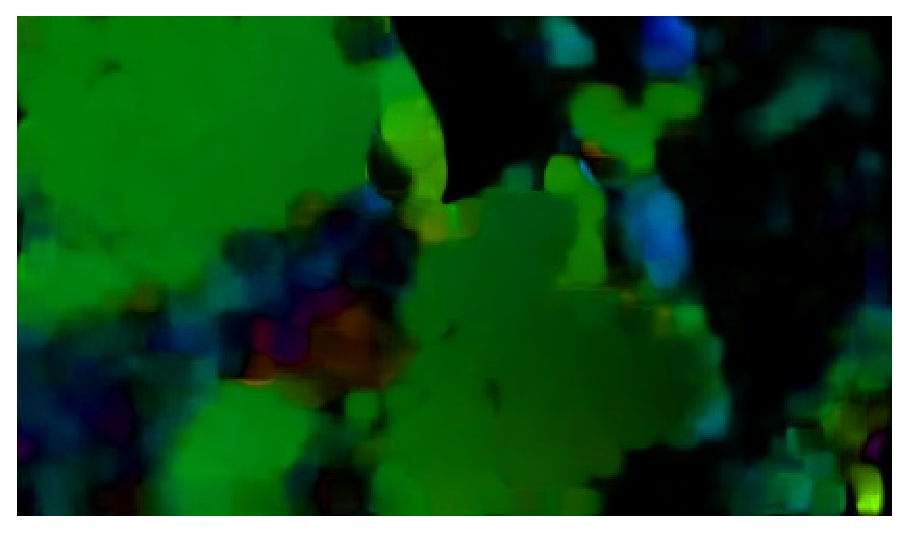
\includegraphics[clip, width=2.5cm]{./Figures/optic_commandmatemate2.eps}
          \hspace{0.0cm} { }
        \end{center}
      \end{minipage}
      \begin{minipage}{0.165\hsize}
        \begin{center}
          
\includegraphics[clip, width=2.5cm]{./Figures/optic_commandmatemate3.eps}
          \hspace{0.0cm} {command-A}
        \end{center}
      \end{minipage}
      \begin{minipage}{0.165\hsize}
        \begin{center}
          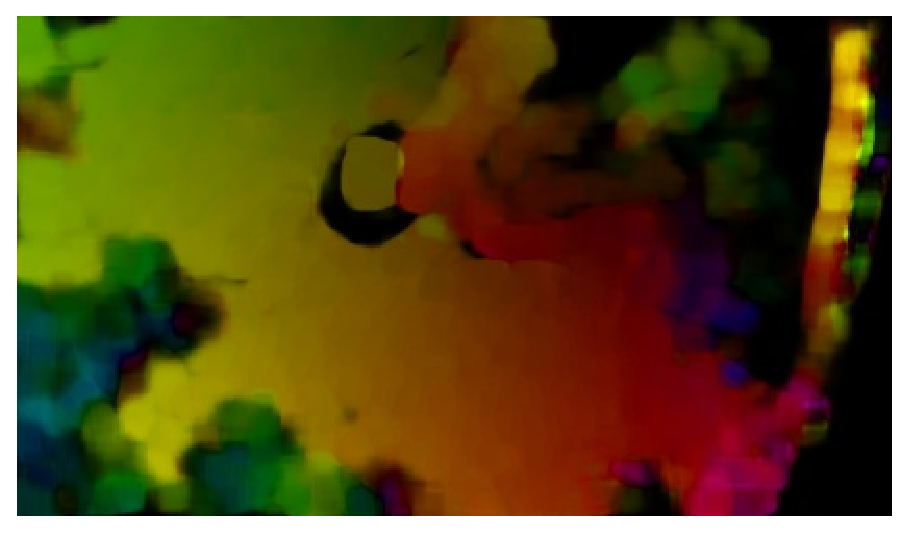
\includegraphics[clip, width=2.5cm]{./Figures/optic_commandmatemate4.eps}
          \hspace{0.1cm} { }
        \end{center}
      \end{minipage}
      \begin{minipage}{0.165\hsize}
        \begin{center}
          
\includegraphics[clip, width=2.5cm]{./Figures/optic_commandmatemate5.eps}
          \hspace{2.2cm} { }
        \end{center}
      \end{minipage}
\\ %%%%%%%%%%%%%%%%%%%%%%%%%%%%%%%%%%

      \begin{minipage}{0.165\hsize}
        \begin{center}
          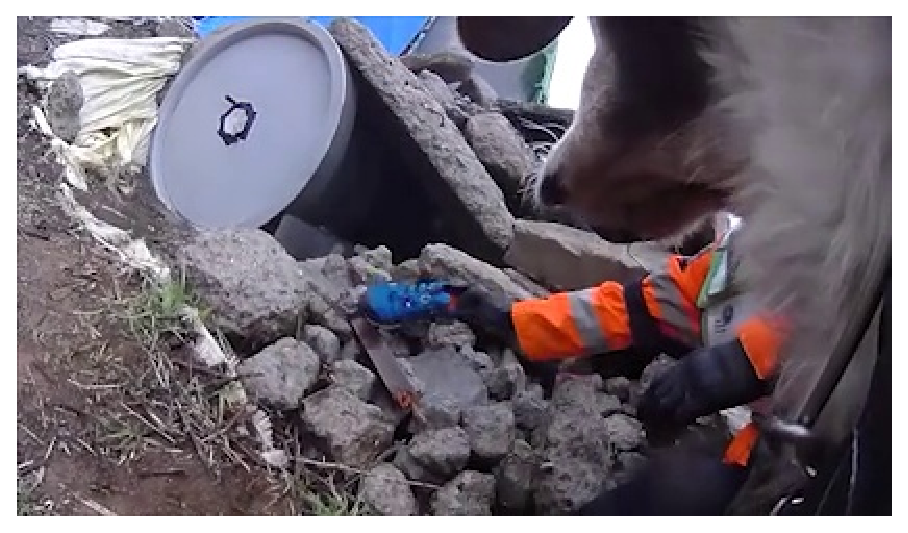
\includegraphics[clip, width=2.5cm]{./Figures/still_commandshoo1.eps}
        \end{center}
      \end{minipage}
      \begin{minipage}{0.165\hsize}
        \begin{center}
          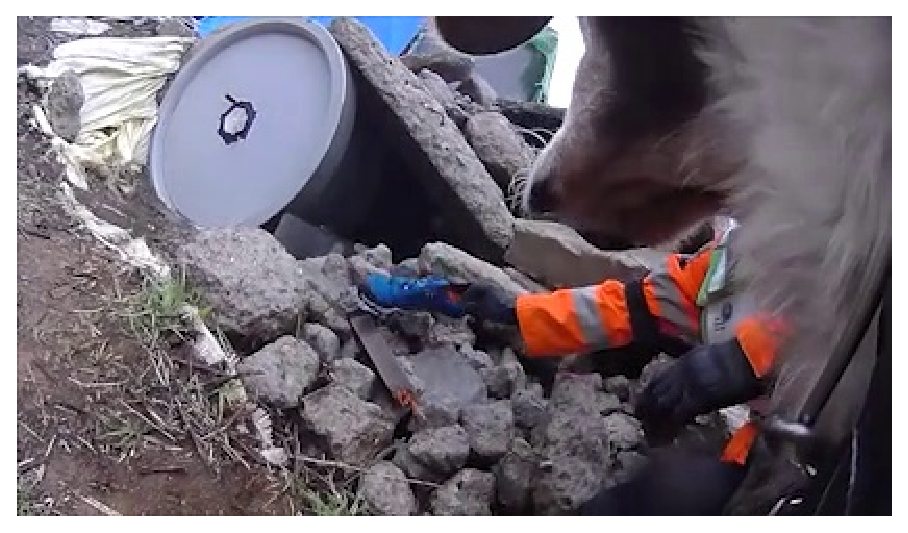
\includegraphics[clip, width=2.5cm]{./Figures/still_commandshoo2.eps}
        \end{center}
      \end{minipage}
      \begin{minipage}{0.165\hsize}
        \begin{center}
          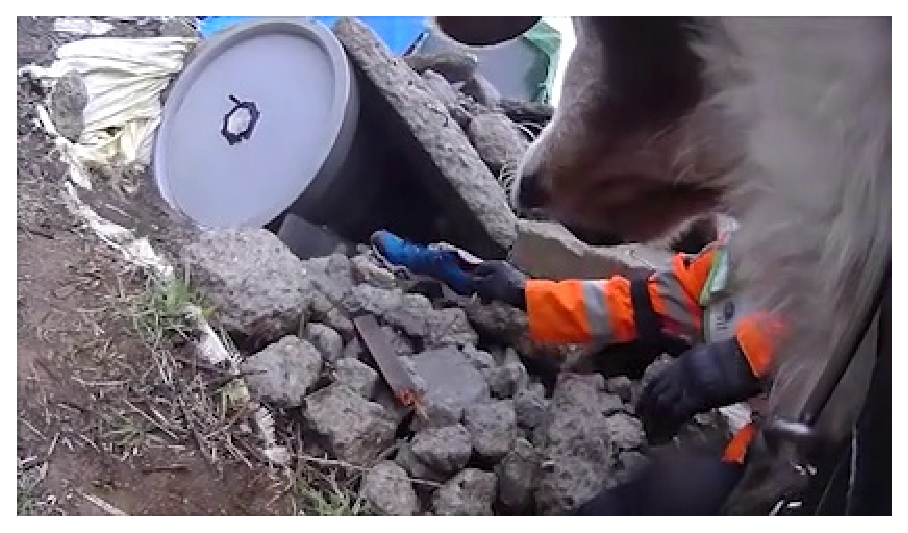
\includegraphics[clip, width=2.5cm]{./Figures/still_commandshoo3.eps}
        \end{center}
      \end{minipage}
      \begin{minipage}{0.165\hsize}
        \begin{center}
          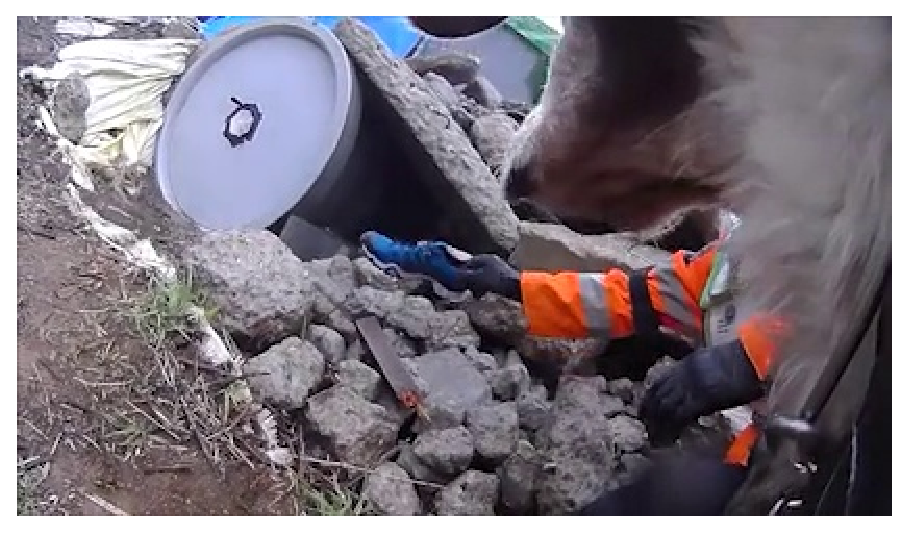
\includegraphics[clip, width=2.5cm]{./Figures/still_commandshoo4.eps}
        \end{center}
      \end{minipage}
      \begin{minipage}{0.165\hsize}
        \begin{center}
          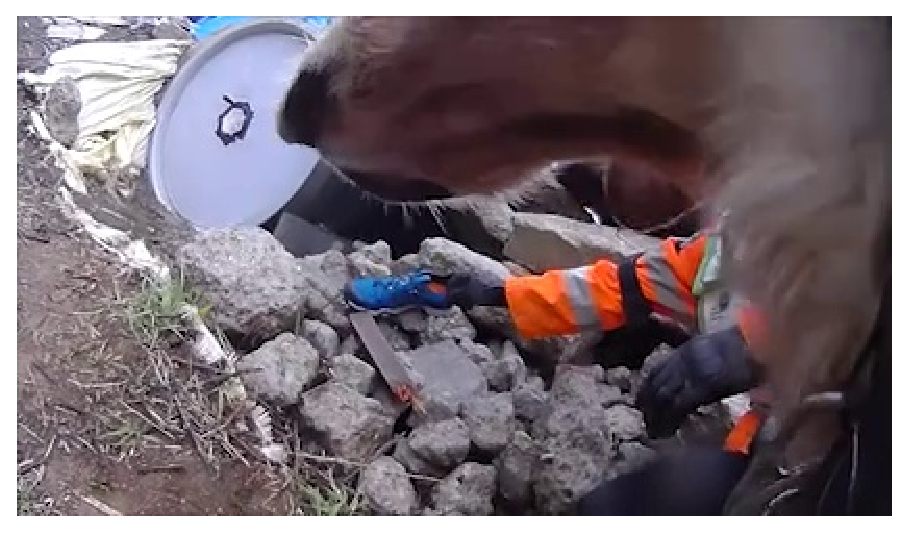
\includegraphics[clip, width=2.5cm]{./Figures/still_commandshoo5.eps}
        \end{center}
      \end{minipage}
      \begin{minipage}{0.165\hsize}
        \begin{center}
          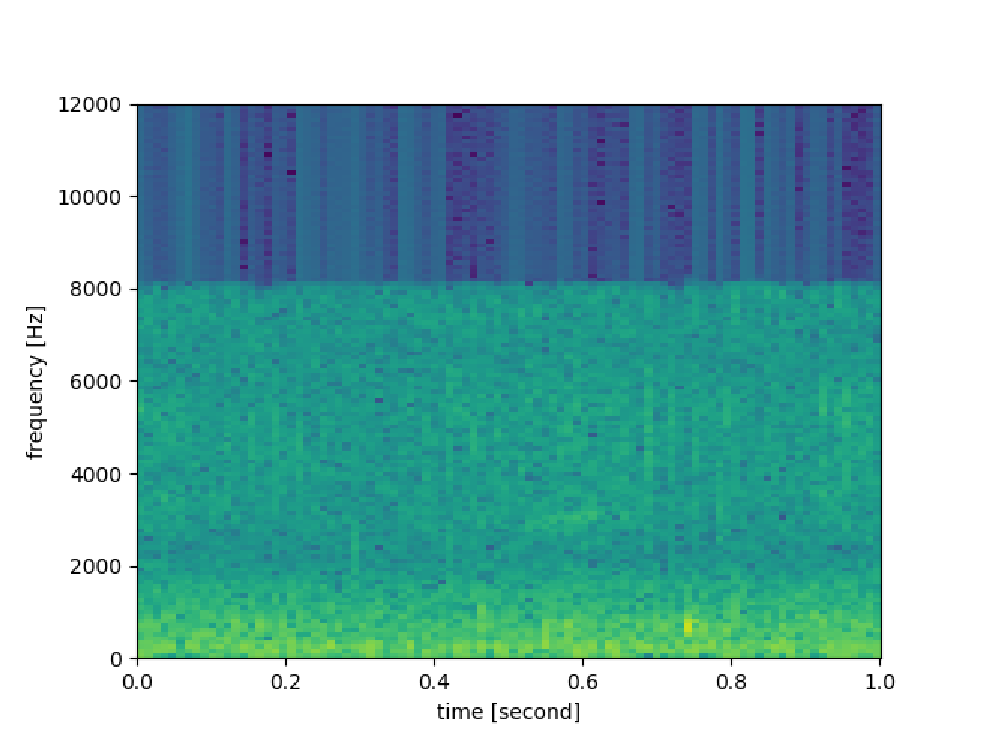
\includegraphics[clip, width=2.5cm]{./Figures/sound_commandshoo.eps}
        \end{center}
      \end{minipage}
\\  %%%%%%%%%%%%%%%%
      \begin{minipage}{0.165\hsize}
        \begin{center}
          
\includegraphics[clip, width=2.5cm]{./Figures/optic_commandshoo1.eps}
          \hspace{0.3cm} { }
        \end{center}
      \end{minipage}
      \begin{minipage}{0.165\hsize}
        \begin{center}
          
\includegraphics[clip, width=2.5cm]{./Figures/optic_commandshoo2.eps}
          \hspace{0.0cm} { }
        \end{center}
      \end{minipage}
      \begin{minipage}{0.165\hsize}
        \begin{center}
          
\includegraphics[clip, width=2.5cm]{./Figures/optic_commandshoo3.eps}
          \hspace{0.0cm} {command-B}
        \end{center}
      \end{minipage}
      \begin{minipage}{0.165\hsize}
        \begin{center}
          
\includegraphics[clip, width=2.5cm]{./Figures/optic_commandshoo4.eps}
          \hspace{0.1cm} { }
        \end{center}
      \end{minipage}
      \begin{minipage}{0.165\hsize}
        \begin{center}
          
\includegraphics[clip, width=2.5cm]{./Figures/optic_commandshoo5.eps}
          \hspace{2.2cm} { }
        \end{center}
      \end{minipage}
    \end{tabular}
    \caption{サイバーレスキュー犬訓練データセットcommandクラス.「待て、待て」と口頭指示されている(A)と指差し指示を受けている(B).}
    \label{command}
\end{figure}

\begin{figure}[H]
    \begin{tabular}{l}

\\ %%%%%%%%%%%%%%%%%%%%%%%%%%%%%%%%%%

      \begin{minipage}{0.165\hsize}
        \begin{center}
          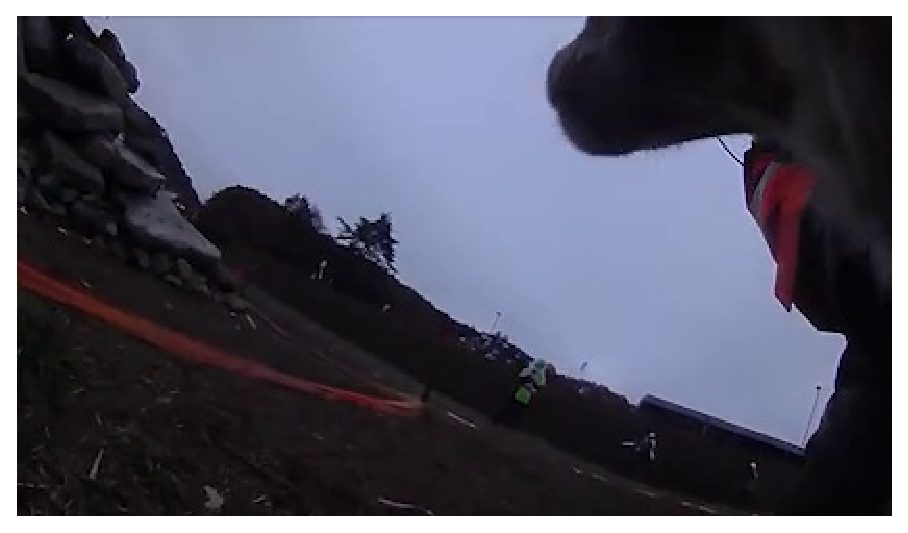
\includegraphics[clip, width=2.5cm]{./Figures/still_eat1.eps}
        \end{center}
      \end{minipage}
      \begin{minipage}{0.165\hsize}
        \begin{center}
          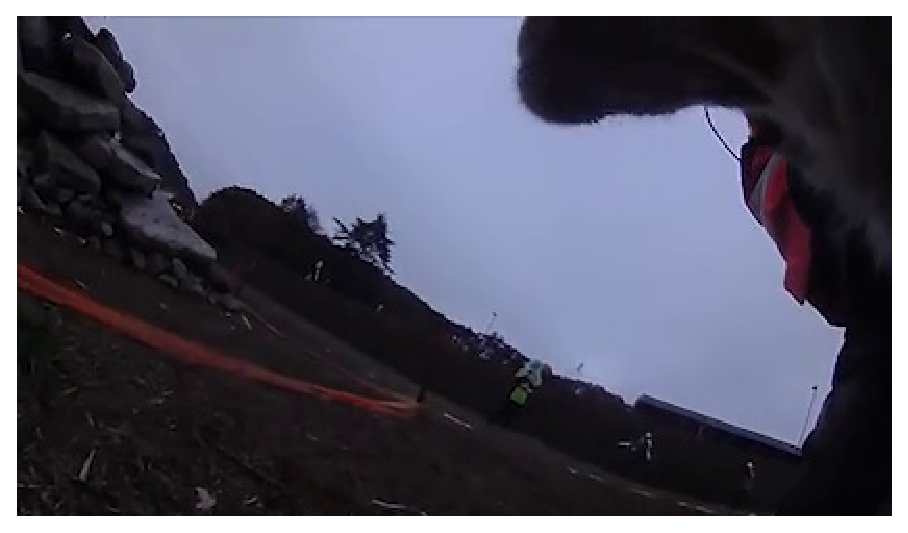
\includegraphics[clip, width=2.5cm]{./Figures/still_eat2.eps}
        \end{center}
      \end{minipage}
      \begin{minipage}{0.165\hsize}
        \begin{center}
          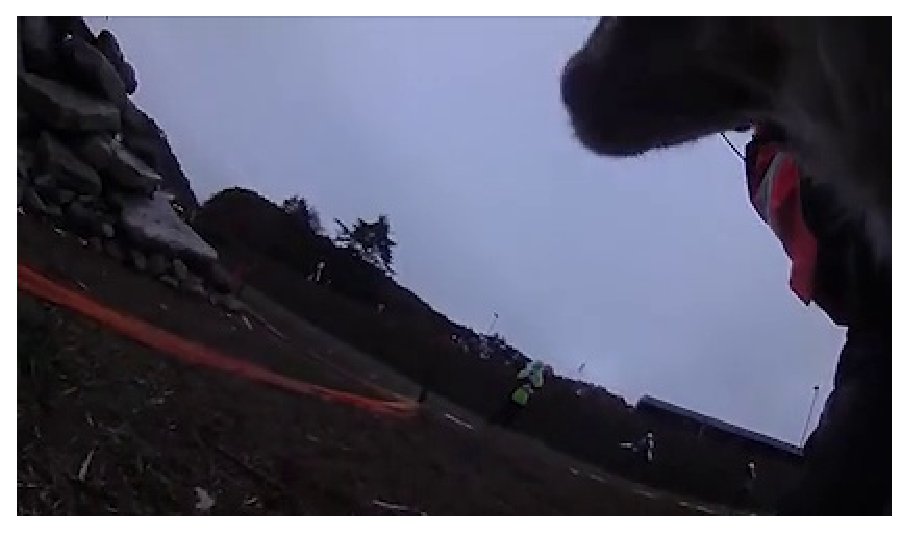
\includegraphics[clip, width=2.5cm]{./Figures/still_eat3.eps}
        \end{center}
      \end{minipage}
      \begin{minipage}{0.165\hsize}
        \begin{center}
          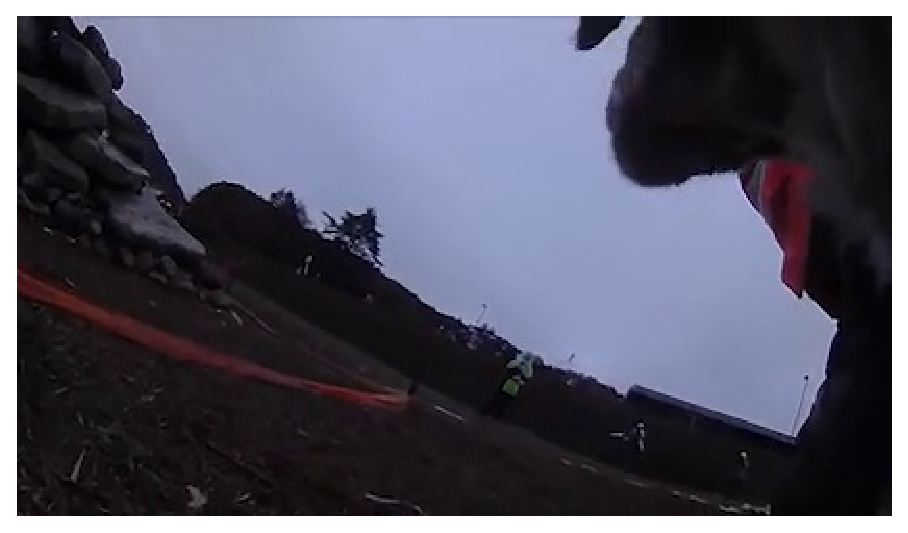
\includegraphics[clip, width=2.5cm]{./Figures/still_eat4.eps}
        \end{center}
      \end{minipage}
      \begin{minipage}{0.165\hsize}
        \begin{center}
          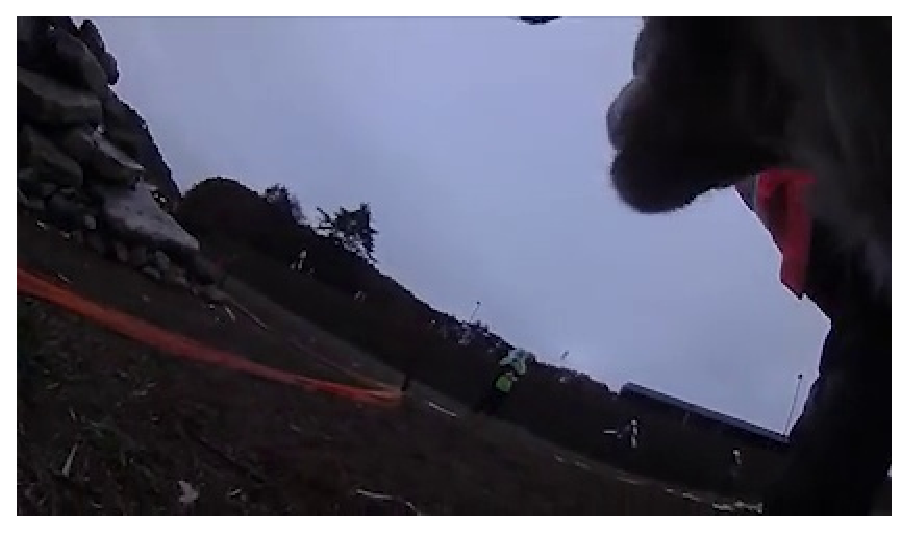
\includegraphics[clip, width=2.5cm]{./Figures/still_eat5.eps}
        \end{center}
      \end{minipage}
      \begin{minipage}{0.165\hsize}
        \begin{center}
          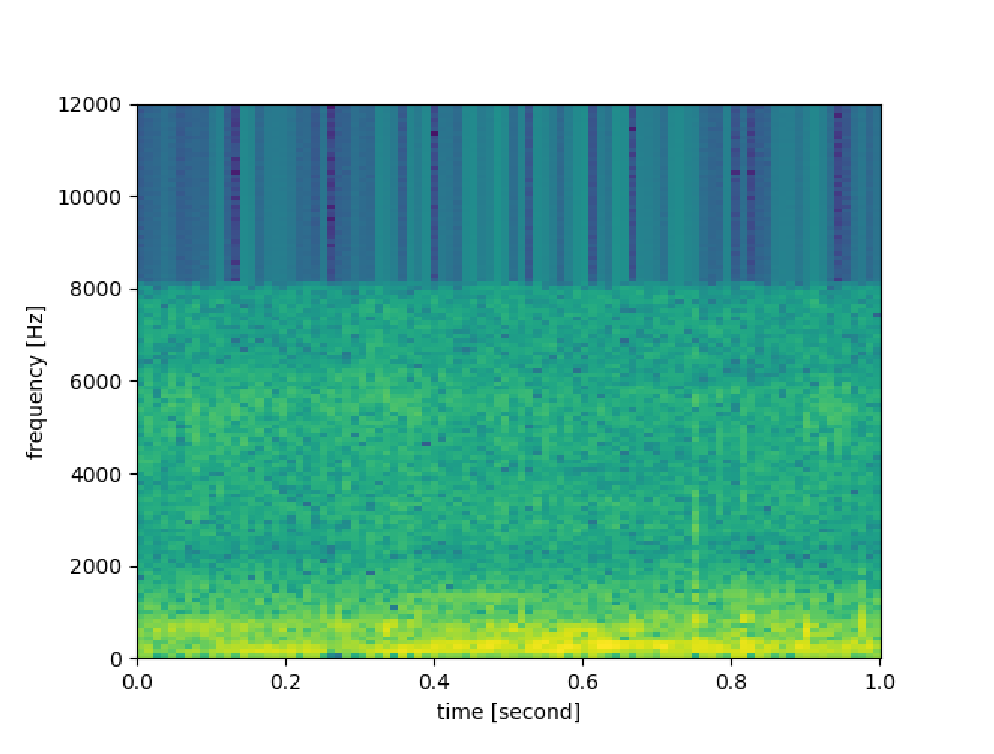
\includegraphics[clip, width=2.5cm]{./Figures/sound_eat.eps}
        \end{center}
      \end{minipage}
\\  %%%%%%%%%%%%%%%%
      \begin{minipage}{0.165\hsize}
        \begin{center}
          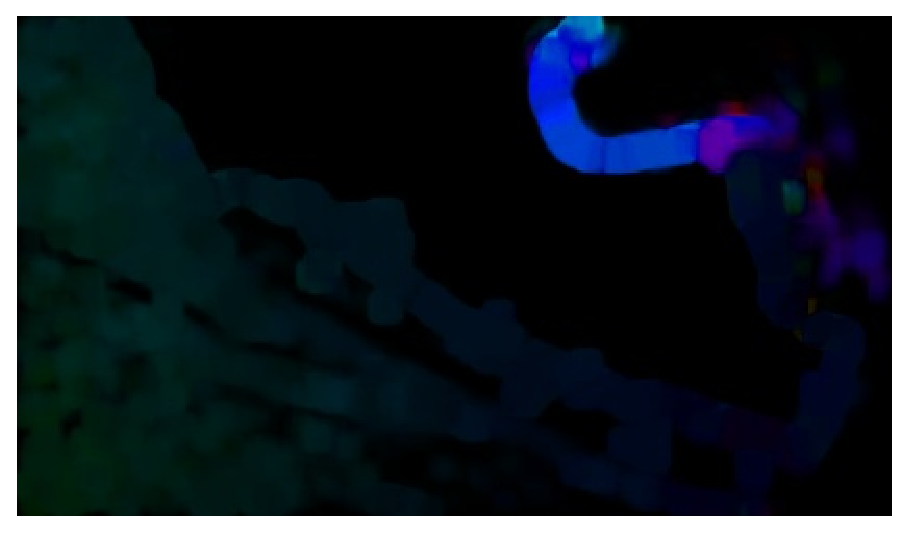
\includegraphics[clip, width=2.5cm]{./Figures/optic_eat1.eps}
          \hspace{0.3cm} { }
        \end{center}
      \end{minipage}
      \begin{minipage}{0.165\hsize}
        \begin{center}
          
\includegraphics[clip, width=2.5cm]{./Figures/optic_eat2.eps}
          \hspace{0.0cm} { }
        \end{center}
      \end{minipage}
      \begin{minipage}{0.165\hsize}
        \begin{center}
          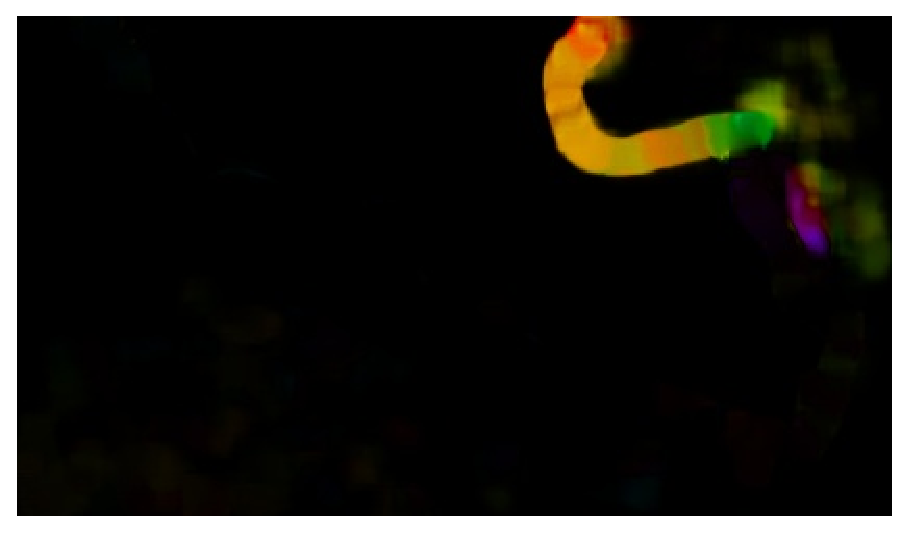
\includegraphics[clip, width=2.5cm]{./Figures/optic_eat3.eps}
          \hspace{0.0cm} {eat}
        \end{center}
      \end{minipage}
      \begin{minipage}{0.165\hsize}
        \begin{center}
          
\includegraphics[clip, width=2.5cm]{./Figures/optic_eat4.eps}
          \hspace{0.1cm} { }
        \end{center}
      \end{minipage}
      \begin{minipage}{0.165\hsize}
        \begin{center}
          
\includegraphics[clip, width=2.5cm]{./Figures/optic_eat5.eps}
          \hspace{2.2cm} { }
        \end{center}
      \end{minipage}
\\ %%%%%%%%%%%%%%%%%%%%%%%%%%%%%%%%%%

      \begin{minipage}{0.165\hsize}
        \begin{center}
          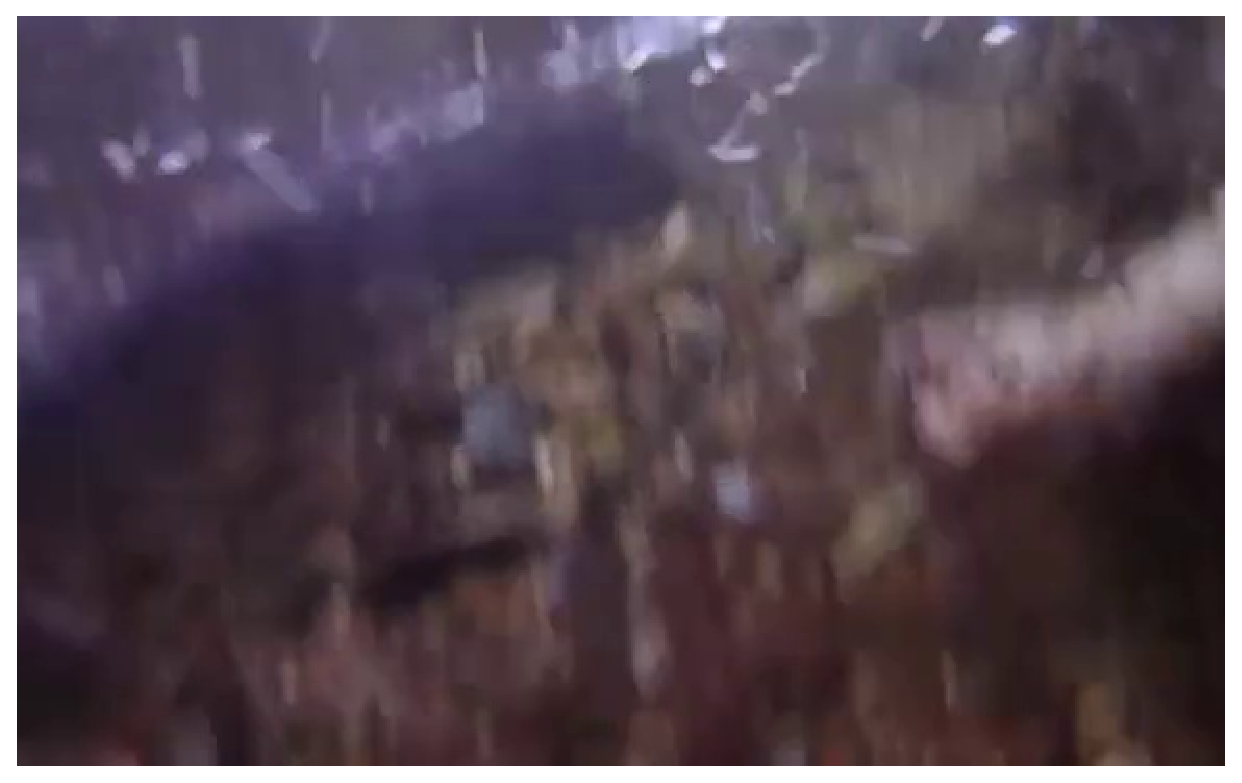
\includegraphics[clip, width=2.5cm]{./Figures/still_drink1.eps}
        \end{center}
      \end{minipage}
      \begin{minipage}{0.165\hsize}
        \begin{center}
          \includegraphics[clip, width=2.5cm]{./Figures/still_drink2.eps}
        \end{center}
      \end{minipage}
      \begin{minipage}{0.165\hsize}
        \begin{center}
          \includegraphics[clip, width=2.5cm]{./Figures/still_drink3.eps}
        \end{center}
      \end{minipage}
      \begin{minipage}{0.165\hsize}
        \begin{center}
          \includegraphics[clip, width=2.5cm]{./Figures/still_drink4.eps}
        \end{center}
      \end{minipage}
      \begin{minipage}{0.165\hsize}
        \begin{center}
          \includegraphics[clip, width=2.5cm]{./Figures/still_drink5.eps}
        \end{center}
      \end{minipage}
      \begin{minipage}{0.165\hsize}
        \begin{center}
          \includegraphics[clip, width=2.5cm]{./Figures/sound_drink.eps}
        \end{center}
      \end{minipage}
\\  %%%%%%%%%%%%%%%%
      \begin{minipage}{0.165\hsize}
        \begin{center}
          \includegraphics[clip, width=2.5cm]{./Figures/optic_drink1.eps}
          \hspace{0.3cm} { }
        \end{center}
      \end{minipage}
      \begin{minipage}{0.165\hsize}
        \begin{center}
          \includegraphics[clip, width=2.5cm]{./Figures/optic_drink2.eps}
          \hspace{0.0cm} { }
        \end{center}
      \end{minipage}
      \begin{minipage}{0.165\hsize}
        \begin{center}
          \includegraphics[clip, width=2.5cm]{./Figures/optic_drink3.eps}
          \hspace{0.0cm} {drink}
        \end{center}
      \end{minipage}
      \begin{minipage}{0.165\hsize}
        \begin{center}
          \includegraphics[clip, width=2.5cm]{./Figures/optic_drink4.eps}
          \hspace{0.1cm} { }
        \end{center}
      \end{minipage}
      \begin{minipage}{0.165\hsize}
        \begin{center}
          \includegraphics[clip, width=2.5cm]{./Figures/optic_drink5.eps}
          \hspace{2.2cm} { }
        \end{center}
      \end{minipage}
    \end{tabular}
    \caption{サイバーレスキュー犬訓練データセットeat-drinkクラス.訓練時にハンドラーから餌を受け取っている(eat)と森林での訓練で川の水を飲んでいる(drink)}
    \label{eat-drink}
\end{figure}

\begin{figure}[H]
    \begin{tabular}{l}

\\ %%%%%%%%%%%%%%%%%%%%%%%%%%%%%%%%%%
     % 0
      \begin{minipage}{0.165\hsize}
        \begin{center}
          \includegraphics[clip, width=2.5cm]{./Figures/still_look1.eps}
        \end{center}
      \end{minipage}
      \begin{minipage}{0.165\hsize}
        \begin{center}
          \includegraphics[clip, width=2.5cm]{./Figures/still_look2.eps}
        \end{center}
      \end{minipage}
      \begin{minipage}{0.165\hsize}
        \begin{center}
          \includegraphics[clip, width=2.5cm]{./Figures/still_look3.eps}
        \end{center}
      \end{minipage}
      \begin{minipage}{0.165\hsize}
        \begin{center}
          \includegraphics[clip, width=2.5cm]{./Figures/still_look4.eps}
        \end{center}
      \end{minipage}
      \begin{minipage}{0.165\hsize}
        \begin{center}
          \includegraphics[clip, width=2.5cm]{./Figures/still_look5.eps}
        \end{center}
      \end{minipage}
      \begin{minipage}{0.165\hsize}
        \begin{center}
          \includegraphics[clip, width=2.5cm]{./Figures/sound_look.eps}
        \end{center}
      \end{minipage}
\\  %%%%%%%%%%%%%%%%
      \begin{minipage}{0.165\hsize}
        \begin{center}
          \includegraphics[clip, width=2.5cm]{./Figures/optic_look1.eps}
          \hspace{0.3cm} { }
        \end{center}
      \end{minipage}
      \begin{minipage}{0.165\hsize}
        \begin{center}
          \includegraphics[clip, width=2.5cm]{./Figures/optic_look2.eps}
          \hspace{0.0cm} { }
        \end{center}
      \end{minipage}
      \begin{minipage}{0.165\hsize}
        \begin{center}
          \includegraphics[clip, width=2.5cm]{./Figures/optic_look3.eps}
          \hspace{2.0cm} {look handler}
        \end{center}
      \end{minipage}
      \begin{minipage}{0.165\hsize}
        \begin{center}
          \includegraphics[clip, width=2.5cm]{./Figures/optic_look4.eps}
          \hspace{0.1cm} { }
        \end{center}
      \end{minipage}
      \begin{minipage}{0.165\hsize}
        \begin{center}
          \includegraphics[clip, width=2.5cm]{./Figures/optic_look5.eps}
          \hspace{2.2cm} { }
        \end{center}
      \end{minipage}
    \end{tabular}
    \caption{サイバーレスキュー犬訓練データセットlook at handlerクラス.}
    \label{lookathandler}
\end{figure}

\begin{figure}[H]
    \begin{tabular}{l}

\\ %%%%%%%%%%%%%%%%%%%%%%%%%%%%%%%%%%
      \begin{minipage}{0.165\hsize}
        \begin{center}
          \includegraphics[clip, width=2.5cm]{./Figures/still_sniffcling1.eps}
        \end{center}
      \end{minipage}
      \begin{minipage}{0.165\hsize}
        \begin{center}
          \includegraphics[clip, width=2.5cm]{./Figures/still_sniffcling2.eps}
        \end{center}
      \end{minipage}
      \begin{minipage}{0.165\hsize}
        \begin{center}
          \includegraphics[clip, width=2.5cm]{./Figures/still_sniffcling3.eps}
        \end{center}
      \end{minipage}
      \begin{minipage}{0.165\hsize}
        \begin{center}
          \includegraphics[clip, width=2.5cm]{./Figures/still_sniffcling4.eps}
        \end{center}
      \end{minipage}
      \begin{minipage}{0.165\hsize}
        \begin{center}
          \includegraphics[clip, width=2.5cm]{./Figures/still_sniffcling5.eps}
        \end{center}
      \end{minipage}
      \begin{minipage}{0.165\hsize}
        \begin{center}
          \includegraphics[clip, width=2.5cm]{./Figures/sound_sniffcling.eps}
        \end{center}
      \end{minipage}
\\  %%%%%%%%%%%%%%%%
      \begin{minipage}{0.165\hsize}
        \begin{center}
          \includegraphics[clip, width=2.5cm]{./Figures/optic_sniffcling1.eps}
          \hspace{0.3cm} { }
        \end{center}
      \end{minipage}
      \begin{minipage}{0.165\hsize}
        \begin{center}
          \includegraphics[clip, width=2.5cm]{./Figures/optic_sniffcling2.eps}
          \hspace{0.0cm} { }
        \end{center}
      \end{minipage}
      \begin{minipage}{0.165\hsize}
        \begin{center}
          \includegraphics[clip, width=2.5cm]{./Figures/optic_sniffcling3.eps}
          \hspace{0.0cm} {cling}
        \end{center}
      \end{minipage}
      \begin{minipage}{0.165\hsize}
        \begin{center}
          \includegraphics[clip, width=2.5cm]{./Figures/optic_sniffcling4.eps}
          \hspace{0.1cm} { }
        \end{center}
      \end{minipage}
      \begin{minipage}{0.165\hsize}
        \begin{center}
          \includegraphics[clip, width=2.5cm]{./Figures/optic_sniffcling5.eps}
          \hspace{2.2cm} { }
        \end{center}
      \end{minipage}
    \end{tabular}
    \caption{サイバーレスキュー犬訓練データセットclingクラス.}
    \label{sniff}
\end{figure}

\begin{figure}[H]
    \begin{tabular}{l}

\\ %%%%%%%%%%%%%%%%%%%%%%%%%%%%%%%%%%

      \begin{minipage}{0.165\hsize}
        \begin{center}
          \includegraphics[clip, width=2.5cm]{./Figures/still_seevictim1.eps}
        \end{center}
      \end{minipage}
      \begin{minipage}{0.165\hsize}
        \begin{center}
          \includegraphics[clip, width=2.5cm]{./Figures/still_seevictim2.eps}
        \end{center}
      \end{minipage}
      \begin{minipage}{0.165\hsize}
        \begin{center}
          \includegraphics[clip, width=2.5cm]{./Figures/still_seevictim3.eps}
        \end{center}
      \end{minipage}
      \begin{minipage}{0.165\hsize}
        \begin{center}
          \includegraphics[clip, width=2.5cm]{./Figures/still_seevictim4.eps}
        \end{center}
      \end{minipage}
      \begin{minipage}{0.165\hsize}
        \begin{center}
          \includegraphics[clip, width=2.5cm]{./Figures/still_seevictim5.eps}
        \end{center}
      \end{minipage}
      \begin{minipage}{0.165\hsize}
        \begin{center}
          \includegraphics[clip, width=2.5cm]{./Figures/sound_seevictim.eps}
        \end{center}
      \end{minipage}
\\  %%%%%%%%%%%%%%%%
      \begin{minipage}{0.165\hsize}
        \begin{center}
          \includegraphics[clip, width=2.5cm]{./Figures/optic_seevictim1.eps}
          \hspace{0.3cm} { }
        \end{center}
      \end{minipage}
      \begin{minipage}{0.165\hsize}
        \begin{center}
          \includegraphics[clip, width=2.5cm]{./Figures/optic_seevictim2.eps}
          \hspace{0.0cm} { }
        \end{center}
      \end{minipage}
      \begin{minipage}{0.165\hsize}
        \begin{center}
          \includegraphics[clip, width=2.5cm]{./Figures/optic_seevictim3.eps}
          \hspace{2.0cm} {see victim}
        \end{center}
      \end{minipage}
      \begin{minipage}{0.165\hsize}
        \begin{center}
          \includegraphics[clip, width=2.5cm]{./Figures/optic_seevictim4.eps}
          \hspace{0.1cm} { }
        \end{center}
      \end{minipage}
      \begin{minipage}{0.165\hsize}
        \begin{center}
          \includegraphics[clip, width=2.5cm]{./Figures/optic_seevictim5.eps}
          \hspace{2.2cm} { }
        \end{center}
      \end{minipage}
    \end{tabular}
    \caption{サイバーレスキュー犬訓練データセットsee victimクラス.}
    \label{seevictim}
\end{figure}

\begin{figure}[H]
    \begin{tabular}{l}


\\ %%%%%%%%%%%%%%%%%%%%%%%%%%%%%%%%%%

      \begin{minipage}{0.165\hsize}
        \begin{center}
          \includegraphics[clip, width=2.5cm]{./Figures/still_shake1.eps}
        \end{center}
      \end{minipage}
      \begin{minipage}{0.165\hsize}
        \begin{center}
          \includegraphics[clip, width=2.5cm]{./Figures/still_shake2.eps}
        \end{center}
      \end{minipage}
      \begin{minipage}{0.165\hsize}
        \begin{center}
          \includegraphics[clip, width=2.5cm]{./Figures/still_shake3.eps}
        \end{center}
      \end{minipage}
      \begin{minipage}{0.165\hsize}
        \begin{center}
          \includegraphics[clip, width=2.5cm]{./Figures/still_shake4.eps}
        \end{center}
      \end{minipage}
      \begin{minipage}{0.165\hsize}
        \begin{center}
          \includegraphics[clip, width=2.5cm]{./Figures/still_shake5.eps}
        \end{center}
      \end{minipage}
      \begin{minipage}{0.165\hsize}
        \begin{center}
          \includegraphics[clip, width=2.5cm]{./Figures/sound_shake.eps}
        \end{center}
      \end{minipage}
\\  %%%%%%%%%%%%%%%%
      \begin{minipage}{0.165\hsize}
        \begin{center}
          \includegraphics[clip, width=2.5cm]{./Figures/optic_shake1.eps}
          \hspace{0.3cm} { }
        \end{center}
      \end{minipage}
      \begin{minipage}{0.165\hsize}
        \begin{center}
          \includegraphics[clip, width=2.5cm]{./Figures/optic_shake2.eps}
          \hspace{0.0cm} { }
        \end{center}
      \end{minipage}
      \begin{minipage}{0.165\hsize}
        \begin{center}
          \includegraphics[clip, width=2.5cm]{./Figures/optic_shake3.eps}
          \hspace{2.0cm} {shake}
        \end{center}
      \end{minipage}
      \begin{minipage}{0.165\hsize}
        \begin{center}
          \includegraphics[clip, width=2.5cm]{./Figures/optic_shake4.eps}
          \hspace{0.1cm} { }
        \end{center}
      \end{minipage}
      \begin{minipage}{0.165\hsize}
        \begin{center}
          \includegraphics[clip, width=2.5cm]{./Figures/optic_shake5.eps}
          \hspace{2.2cm} { }
        \end{center}
      \end{minipage}
    \end{tabular}
    \caption{サイバーレスキュー犬訓練データセットshakeクラス.}
    \label{shake}
\end{figure}

\begin{figure}[H]
    \begin{tabular}{l}


\\ %%%%%%%%%%%%%%%%%%%%%%%%%%%%%%%%%%


    \end{tabular}
\end{figure}
\begin{figure}[htbp]
    \begin{tabular}{l}
     % 0
      \begin{minipage}{0.165\hsize}
        \begin{center}
          \includegraphics[clip, width=2.5cm]{./Figures/still_stop1-1.eps}
        \end{center}
      \end{minipage}
      \begin{minipage}{0.165\hsize}
        \begin{center}
          \includegraphics[clip, width=2.5cm]{./Figures/still_stop1-2.eps}
        \end{center}
      \end{minipage}
      \begin{minipage}{0.165\hsize}
        \begin{center}
          \includegraphics[clip, width=2.5cm]{./Figures/still_stop1-3.eps}
        \end{center}
      \end{minipage}
      \begin{minipage}{0.165\hsize}
        \begin{center}
          \includegraphics[clip, width=2.5cm]{./Figures/still_stop1-4.eps}
        \end{center}
      \end{minipage}
      \begin{minipage}{0.165\hsize}
        \begin{center}
          \includegraphics[clip, width=2.5cm]{./Figures/still_stop1-5.eps}
        \end{center}
      \end{minipage}
      \begin{minipage}{0.165\hsize}
        \begin{center}
          \includegraphics[clip, width=2.5cm]{./Figures/sound_stop.eps}
        \end{center}
      \end{minipage}
\\  %%%%%%%%%%%%%%%%
      \begin{minipage}{0.165\hsize}
        \begin{center}
          \includegraphics[clip, width=2.5cm]{./Figures/optic_stop1-1.eps}
          \hspace{0.3cm} { }
        \end{center}
      \end{minipage}
      \begin{minipage}{0.165\hsize}
        \begin{center}
          \includegraphics[clip, width=2.5cm]{./Figures/optic_stop1-2.eps}
          \hspace{0.0cm} { }
        \end{center}
      \end{minipage}
      \begin{minipage}{0.165\hsize}
        \begin{center}
          \includegraphics[clip, width=2.5cm]{./Figures/optic_stop1-3.eps}
          \hspace{2.0cm} {stop-A}
        \end{center}
      \end{minipage}
      \begin{minipage}{0.165\hsize}
        \begin{center}
          \includegraphics[clip, width=2.5cm]{./Figures/optic_stop1-4.eps}
          \hspace{0.1cm} { }
        \end{center}
      \end{minipage}
      \begin{minipage}{0.165\hsize}
        \begin{center}
          \includegraphics[clip, width=2.5cm]{./Figures/optic_stop1-5.eps}
          \hspace{2.2cm} { }
        \end{center}
      \end{minipage}
\\ %%%%%%%%%%%%%%%%%%%%%%%%%%%%%%%%%%
      \begin{minipage}{0.165\hsize}
        \begin{center}
          \includegraphics[clip, width=2.5cm]{./Figures/still_stop2-1.eps}
        \end{center}
      \end{minipage}
      \begin{minipage}{0.165\hsize}
        \begin{center}
          \includegraphics[clip, width=2.5cm]{./Figures/still_stop2-2.eps}
        \end{center}
      \end{minipage}
      \begin{minipage}{0.165\hsize}
        \begin{center}
          \includegraphics[clip, width=2.5cm]{./Figures/still_stop2-3.eps}
        \end{center}
      \end{minipage}
      \begin{minipage}{0.165\hsize}
        \begin{center}
          \includegraphics[clip, width=2.5cm]{./Figures/still_stop2-4.eps}
        \end{center}
      \end{minipage}
      \begin{minipage}{0.165\hsize}
        \begin{center}
          \includegraphics[clip, width=2.5cm]{./Figures/still_stop2-5.eps}
        \end{center}
      \end{minipage}
      \begin{minipage}{0.165\hsize}
        \begin{center}
          \includegraphics[clip, width=2.5cm]{./Figures/sound_stop2.eps}
        \end{center}
      \end{minipage}
\\  %%%%%%%%%%%%%%%%
      \begin{minipage}{0.165\hsize}
        \begin{center}
          \includegraphics[clip, width=2.5cm]{./Figures/optic_stop2-1.eps}
          \hspace{0.3cm} { }
        \end{center}
      \end{minipage}
      \begin{minipage}{0.165\hsize}
        \begin{center}
          \includegraphics[clip, width=2.5cm]{./Figures/optic_stop2-2.eps}
          \hspace{0.0cm} { }
        \end{center}
      \end{minipage}
      \begin{minipage}{0.165\hsize}
        \begin{center}
          \includegraphics[clip, width=2.5cm]{./Figures/optic_stop2-3.eps}
          \hspace{2.0cm} {stop-B}
        \end{center}
      \end{minipage}
      \begin{minipage}{0.165\hsize}
        \begin{center}
          \includegraphics[clip, width=2.5cm]{./Figures/optic_stop2-4.eps}
          \hspace{0.1cm} { }
        \end{center}
      \end{minipage}
      \begin{minipage}{0.165\hsize}
        \begin{center}
          \includegraphics[clip, width=2.5cm]{./Figures/optic_stop2-5.eps}
          \hspace{2.2cm} { }
        \end{center}
      \end{minipage}
    \end{tabular}
    \caption{サイバーレスキュー犬訓練データセットstopクラス.}
    \label{stop}
\end{figure}

\begin{figure}[H]
    \begin{tabular}{l}


\\ %%%%%%%%%%%%%%%%%%%%%%%%%%%%%%%%%%

      \begin{minipage}{0.165\hsize}
        \begin{center}
          \includegraphics[clip, width=2.5cm]{./Figures/still_run1.eps}
        \end{center}
      \end{minipage}
      \begin{minipage}{0.165\hsize}
        \begin{center}
          \includegraphics[clip, width=2.5cm]{./Figures/still_run2.eps}
        \end{center}
      \end{minipage}
      \begin{minipage}{0.165\hsize}
        \begin{center}
          \includegraphics[clip, width=2.5cm]{./Figures/still_run3.eps}
        \end{center}
      \end{minipage}
      \begin{minipage}{0.165\hsize}
        \begin{center}
          \includegraphics[clip, width=2.5cm]{./Figures/still_run4.eps}
        \end{center}
      \end{minipage}
      \begin{minipage}{0.165\hsize}
        \begin{center}
          \includegraphics[clip, width=2.5cm]{./Figures/still_run5.eps}
        \end{center}
      \end{minipage}
      \begin{minipage}{0.165\hsize}
        \begin{center}
          \includegraphics[clip, width=2.5cm]{./Figures/sound_run.eps}
        \end{center}
      \end{minipage}
\\  %%%%%%%%%%%%%%%%
      \begin{minipage}{0.165\hsize}
        \begin{center}
          \includegraphics[clip, width=2.5cm]{./Figures/optic_run1.eps}
          \hspace{0.3cm} { }
        \end{center}
      \end{minipage}
      \begin{minipage}{0.165\hsize}
        \begin{center}
          \includegraphics[clip, width=2.5cm]{./Figures/optic_run2.eps}
          \hspace{0.0cm} { }
        \end{center}
      \end{minipage}
      \begin{minipage}{0.165\hsize}
        \begin{center}
          \includegraphics[clip, width=2.5cm]{./Figures/optic_run3.eps}
          \hspace{2.0cm} {run}
        \end{center}
      \end{minipage}
      \begin{minipage}{0.165\hsize}
        \begin{center}
          \includegraphics[clip, width=2.5cm]{./Figures/optic_run4.eps}
          \hspace{0.1cm} { }
        \end{center}
      \end{minipage}
      \begin{minipage}{0.165\hsize}
        \begin{center}
          \includegraphics[clip, width=2.5cm]{./Figures/optic_run5.eps}
          \hspace{2.2cm} { }
        \end{center}
      \end{minipage}
    \end{tabular}
    \caption{サイバーレスキュー犬訓練データセットrunクラス.}
    \label{run}
\end{figure}

\begin{figure}[H]
    \begin{tabular}{l}


\\ %%%%%%%%%%%%%%%%%%%%%%%%%%%%%%%%%%

      \begin{minipage}{0.165\hsize}
        \begin{center}
          \includegraphics[clip, width=2.5cm]{./Figures/still_walk1.eps}
        \end{center}
      \end{minipage}
      \begin{minipage}{0.165\hsize}
        \begin{center}
          \includegraphics[clip, width=2.5cm]{./Figures/still_walk2.eps}
        \end{center}
      \end{minipage}
      \begin{minipage}{0.165\hsize}
        \begin{center}
          \includegraphics[clip, width=2.5cm]{./Figures/still_walk3.eps}
        \end{center}
      \end{minipage}
      \begin{minipage}{0.165\hsize}
        \begin{center}
          \includegraphics[clip, width=2.5cm]{./Figures/still_walk4.eps}
        \end{center}
      \end{minipage}
      \begin{minipage}{0.165\hsize}
        \begin{center}
          \includegraphics[clip, width=2.5cm]{./Figures/still_walk5.eps}
        \end{center}
      \end{minipage}
      \begin{minipage}{0.165\hsize}
        \begin{center}
          \includegraphics[clip, width=2.5cm]{./Figures/sound_walk.eps}
        \end{center}
      \end{minipage}
\\  %%%%%%%%%%%%%%%%
      \begin{minipage}{0.165\hsize}
        \begin{center}
          \includegraphics[clip, width=2.5cm]{./Figures/optic_walk1.eps}
          \hspace{0.3cm} { }
        \end{center}
      \end{minipage}
      \begin{minipage}{0.165\hsize}
        \begin{center}
          \includegraphics[clip, width=2.5cm]{./Figures/optic_walk2.eps}
          \hspace{0.0cm} { }
        \end{center}
      \end{minipage}
      \begin{minipage}{0.165\hsize}
        \begin{center}
          \includegraphics[clip, width=2.5cm]{./Figures/optic_walk3.eps}
          \hspace{2.0cm} {walk-trot}
        \end{center}
      \end{minipage}
      \begin{minipage}{0.165\hsize}
        \begin{center}
          \includegraphics[clip, width=2.5cm]{./Figures/optic_walk4.eps}
          \hspace{0.1cm} { }
        \end{center}
      \end{minipage}
      \begin{minipage}{0.165\hsize}
        \begin{center}
          \includegraphics[clip, width=2.5cm]{./Figures/optic_walk5.eps}
          \hspace{2.2cm} { }
        \end{center}
      \end{minipage}
\\ %%%%%%%%%%%%%%%%%%%%%%%%%%%%%%%%%%
    \end{tabular}
    \caption{サイバーレスキュー犬訓練データセットwalk-trotクラス}
    \label{walk-trot}
\end{figure}
%    \caption{サイバーレスキュー犬訓練データセット オプティカルフロー画像}
%    \label{cyberdataset_optical}
%    \caption{サイバーレスキュー犬訓練データセット サウンドスペクトログラム}
%    \label{cyberdataset_spectrum}


\subsection{データ整形}
本研究では,提供されたサイバーレスキュー犬訓練データを整形し,クラス毎に短く切り出したクリップセット/フレーム毎に切り出した画像セット/フレーム毎に計算したoptical flow画像セット/フレームに合わせて一定時間毎に切り出した音声セットをそれぞれ作成した.
データを整形して複数セットを作成したのち,さらにラベルのないフレームなどを排除してから,動画に戻した際に6fpsとなる量に学習データを間引いた.
30fps近い動画をフレーム毎に学習すると,直近のフレームに対して過度に反応する恐れがあるため,この処理で過学習を防ぐ狙いがある.
整形・サンプリングによって,学習および評価に使った総フレーム数は14581枚となった.
%この範囲でラベル付けされたクラス毎の回数は~表\ref{cyberdataset_label}に示した.
%静止画のみでの音声付き動画のクラス特徴の表現は困難であるため、整形した動画的特徴,音声的特徴とをそれぞれ~図\ref{cyberdataset_img}に示す.
\subsubsection{動画整形}
提供されたデータ映像は犬一人称視点映像,ハンドラー視点映像,第三者視点映像が横並びに結合(図~\ref{concat_movie})されていたため,これは犬一人称視点映像のみを切り出した.
また,提供された7本の動画にはハンドラー視点がないものや,加えて,結合時にノイズが入ったと思われるものが混在したものがそれぞれ存在したため画像サイズが不揃いであった.ノイズの入った第三者視点のない動画について,図~\ref{noizy_movie}にその例を示す.
これについて,ノイズ部分は切り取ったが比率は揃えなかった.
ノイズは学習に悪影響を与えること,微細なアスペクト比のずれは学習の際に吸収されること,アスペクト比をそろえる際に必要性の有無を判断できない情報が切り取られることをその判断理由とする.
このようにして整形した動画を$V$とする.
\begin{figure}[htbp]
%  \begin{center}
    \begin{tabular}{c}
      \begin{minipage}{0.18\hsize}
        \begin{center}
          \includegraphics[clip, width=12cm]{./Figures/2015_gonta_1.eps}
          %\hspace{0.3cm} { }
        \end{center}
      \end{minipage}
\\
      \begin{minipage}{0.18\hsize}
        \begin{center}
          \includegraphics[clip, width=12cm]{./Figures/2015_gonta_2.eps}
          %\hspace{0.3cm} { }
        \end{center}
      \end{minipage}
\\
      \begin{minipage}{0.18\hsize}
        \begin{center}
          \includegraphics[clip, width=12cm]{./Figures/2015_gonta_3.eps}
          %\hspace{0.3cm} { }
        \end{center}
      \end{minipage}
    \end{tabular}
    \caption{犬一人称視点,第三者視点の結合された動画.ハンドラー視点がなく,犬一人称視点の動画の画面左端一帯に黒いノイズが入っているパターン.ノイズを合わせて1280x360pixelで,犬一人称視点を切り出すと比率は16:9だがノイズを取り除くと比率は崩れる.}
    \label{noizy_movie}
%  \end{center}
\end{figure}






\subsubsection{クリップセット}
$V$からラベル毎にクリップ群を切り出すと,アノテーションが単一のフレームと複数被るフレームが同じクリップを介して存在する.
ただし,同じ箇所から別々のラベルを切り出した際に全く等しく被ることはない.
本研究において,クリップ群を作成する目的はそのフレーム間の平均画像を作成することにある.
フレーム間の平均をとる際にそのフレームの多少の前後で結果が異なるため,その差異の学習を期待して別クリップに同じフレームが重複して現れる問題を無視した.
このクリップセットから計算したフレーム間平均画像を図~\ref{resque_mean}に示す.


\begin{figure}[H]
  \begin{center}
    \begin{tabular}{c}
     % 0
      \begin{minipage}{0.18\hsize}
        \begin{center}
          \includegraphics[clip, width=2.5cm]{./Figures/resque_mean1.eps}
          \hspace{0.3cm} { }
        \end{center}
      \end{minipage}
      \begin{minipage}{0.18\hsize}
        \begin{center}
          \includegraphics[clip, width=2.5cm]{./Figures/resque_mean1.eps}
          \hspace{0.3cm} { }
        \end{center}
      \end{minipage}
      \begin{minipage}{0.18\hsize}
        \begin{center}
          \includegraphics[clip, width=2.5cm]{./Figures/resque_mean1.eps}
          \hspace{2.0cm} {}
        \end{center}
      \end{minipage}
      \begin{minipage}{0.18\hsize}
        \begin{center}
          \includegraphics[clip, width=2.5cm]{./Figures/resque_mean1.eps}
          \hspace{0.1cm} { }
        \end{center}
      \end{minipage}
      \begin{minipage}{0.18\hsize}
        \begin{center}
          \includegraphics[clip, width=2.5cm]{./Figures/resque_mean5.eps}
          \hspace{0.2cm} { }
        \end{center}
      \end{minipage}
    \end{tabular}
    \caption{クリップセットから計算したフレーム間平均画像.}
    \label{resque_mean}
  \end{center}
\end{figure}

\subsubsection{フレーム毎切り抜き画像セット・optical flow画像セット}
フレーム毎に切り出した画像には,そのフレームの時間点にアノテーションされているラベルをそのまま用いた.

optical flowの計算にはPythonのオープンソースライブラリであるOpenCVを用いた.なお,利用したバージョンはpython3.6,OpenCV3.3.1である.
元のRGB動画のフレーム$F_t$と$F_{t+1}$から求まるoptical frame画像を$O_t$とした際に,$O_t$には$F_t$と同じラベルを紐付けた.


\subsubsection{音声セット}
フレーム毎切り抜き画像セットに対応する音声を切り出した.
音声データ$S_t$は,$F_t$を中央において前後15フレーム分の長さとした(式~\ref{sound_length}).
%\[S_t = f(F_{t-15}, F_{t+15}) \label{sound_length}\]
\begin{equation}
\label{sound_length}
S_t = f(F_{t-15}, F_{t+15})
\end{equation}

動画は29.97fpsであるため,31フレームのこれは約1秒に当たる.
動画あるいは音声から実際に犬の行動を推定する場合を想定すると,1秒は短すぎず現実的で取り扱いやすい時間であり,特徴を取り出すにもコストが低いため実験にも適している.


\section{DogCentric Activity Dataset (DCAD)}
4頭の犬の背中にGoProカメラを取り付けて散歩をした動画を単一クラス分けしたデータセット~(図\ref{DCAD_img}).動画は320 x 240 解像度,48 frames per secondで撮影されている.
これは犬の行動を切り出した数秒の動画群で構成される.1つの動画につき1つの行動ラベルが付与されており,これをクリップと呼ぶ.
行動のクラスは10種類(
横断前の待機: Car, 水分の摂取: Drink, 手渡しでの食事: Feed, 左を向く: Look at left, 右を向く: Look at right, 人間が犬を撫でる: Pet, ボールで遊ぶ: Play with ball, 身体をブルブルと振る: Shake, 何かの匂いを嗅ぐ: Sniff, 歩く: Walk
)あり,それぞれ合わせて209クリップになる~(表\ref{DCADlabel}).
散歩する地域やコースは犬毎に異なるが,全ての犬に10クラスのクリップが用意されている.
DCADをラベル毎に図~\ref{DCAD_image}に示す.

本研究ではマルチクラス推定を行うが,DCADはシングルクラス分類のためのデータセットであるため比較に用いることができない.
規模が小さいことから,本実験の前の予備実験にこれを用いた.
\begin{table}[tb]
 \centering
 \caption{DogCentric Activity Dataset 内訳}\label{DCADlabel}
% \scalebox{1.00}[1.00]{
  \begin{tabular}{|l||c|c|c|c|c|c|c|c|c|c|}
   \hline \hline
   Activity& Car &Drink& Feed& Left&Right& Pet & Ball&Shake&Sniff&Walk \\ \hline
   Clips   &   26&   10&   25&   21&   17&   25&   14&   19&   27&   25\\ \hline
  \end{tabular}
% }

\end{table}

\begin{figure}[htbp]
  \begin{center}
    \begin{tabular}{c}
     % 0
      \begin{minipage}{0.18\hsize}
        \begin{center}
          \includegraphics[clip, width=2.5cm]{./Figures/HC005.eps}
          \hspace{0.3cm} { }
        \end{center}
      \end{minipage}
      \begin{minipage}{0.18\hsize}
        \begin{center}
          \includegraphics[clip, width=2.5cm]{./Figures/HC006.eps}
          \hspace{0.3cm} { }
        \end{center}
      \end{minipage}

      % 2
      \begin{minipage}{0.18\hsize}
        \begin{center}
          \includegraphics[clip, width=2.5cm]{./Figures/HC007.eps}
          \hspace{2.0cm} {Car}
        \end{center}
      \end{minipage}

      % 4
      \begin{minipage}{0.18\hsize}
        \begin{center}
          \includegraphics[clip, width=2.5cm]{./Figures/HC008.eps}
          \hspace{0.1cm} { }
        \end{center}
      \end{minipage}
      % 5
      \begin{minipage}{0.18\hsize}
        \begin{center}
          \includegraphics[clip, width=2.5cm]{./Figures/HC009.eps}
          \hspace{0.2cm} { }
        \end{center}
      \end{minipage}
\\
     \begin{minipage}{0.18\hsize}
      \begin{center}
       \includegraphics[clip, width=2.5cm]{./Figures/KL001.eps}
       \hspace{0.3cm} { }
      \end{center}
     \end{minipage}
     \begin{minipage}{0.18\hsize}
      \begin{center}
       \includegraphics[clip, width=2.5cm]{./Figures/KL002.eps}
       \hspace{0.3cm} { }
      \end{center}
     \end{minipage}
     \begin{minipage}{0.18\hsize}
      \begin{center}
       \includegraphics[clip, width=2.5cm]{./Figures/KL003.eps}
       \hspace{0.1cm} {Look\_at\_Left}
      \end{center}
     \end{minipage}
     \begin{minipage}{0.18\hsize}
      \begin{center}
       \includegraphics[clip, width=2.5cm]{./Figures/KL004.eps}
       \hspace{1.3cm} { }
      \end{center}
     \end{minipage}
     \begin{minipage}{0.18\hsize}
      \begin{center}
       \includegraphics[clip, width=2.5cm]{./Figures/KL005.eps}
       \hspace{1.6cm} { }
      \end{center}
     \end{minipage}

    \end{tabular}
    \caption{DogCentric Activity Dataset}
    \label{DCAD_image}
  \end{center}
\end{figure}

